\documentclass[final,3p,times,twocolumn]{elsarticle}
\usepackage{amssymb}
\usepackage[fleqn]{amsmath}
\usepackage{graphicx}
\usepackage{footnote}
\usepackage{graphicx}
\usepackage{array,booktabs}
%\usepackage{algorithm}
\usepackage{algorithmic,algorithm}
\usepackage{pbox}
%\usepackage[noend]{algpseudocode}
\DeclareMathOperator{\argmin}{argmin}
\usepackage{enumitem}
\usepackage{color}
\usepackage{hyperref}
\setlength\parindent{0pt}
\newlength\myindent % define a new length \myindent
\setlength\myindent{2em} % assign the length 2em to \myindet
\newcommand\bindent{%
  \begingroup % starts a group (to keep changes local)
  \setlength{\itemindent}{\myindent} % set itemindent (algorithmic internally uses a list) to the value of \mylength
  \addtolength{\algorithmicindent}{\myindent} % adds \mylength to the default indentation used by algorithmic
}
\newcommand\eindent{\endgroup} % closes a group
\setlength\parskip{\baselineskip}
\journal{MPhil in Scientific Computing}

\begin{document}

\begin{frontmatter}

\title{Probabilistic Decision Trees for binary classification on the Higgs dataset}
\author{Vidhi Lalchand}
\address{Cavendish Laboratory, Department of Physics, J J Thomson Avenue, Cambridge. CB3 0HE}

\begin{abstract}
This paper studies the decision tree (DT) approach to a binary classification problem. A well-calibrated estimate of class membership is needed in many supervised learning applications. Decision trees are not probabilistic models per se but can be extended to give reliable probability estimates. In this paper we propose extending the decision tree output to give calibrated probability estimates. This is implemented as a post-processing step applied to the raw score of the DT algorithm. The implementation uses the scikit-learn package in python \cite{SKLEARN} which implements an optimized version of the CART (Classification and Regression Trees) algorithm.

The extended decision tree, \textit{p-tree} (abbreviates \textit{probability tree}) is used as a machine learning tool for classifying atomic collisions in the Higgs dataset. The dataset has labelled samples belonging to two classes - `signal' and `background'. The signal class represents collisions that indicate the presence of a Higgs and the background class represents collisions that results in the creation of particles which are uninteresting from a Higgs perspective. The performance of the classifier in this context is assessed on the basis of a physics motivated metric called the \textit{Approximate Median Significance} score (AMS for short). One of the goals of the paper is to demonstrate the sensitivity of the AMS objective to the probability estimates produced by the classifier. Finally, the DT approach is contrasted with the parametric SVM approach 
for the binary classification task in the Higgs dataset. This paper also includes a literature review discussing the most successful machine learning approaches on the Higgs dataset. 

\end{abstract}
\end{frontmatter}
\section{Background}

In 2012, the ATLAS\footnote{A Toroidal LHC Apparatus} and the CMS\footnote{Compact Muon Solenoid} experiment observed a new particle in the proton-proton collisions at the LHC (Large Hadron Collider) in CERN. The discovery had a statistical significance of 5$\sigma$ (five-sigma). Five-sigma corresponds to a p-value of $3*10^-7$, or a 1 in 3.5 million chance that the results obtained were purely due to chance. In essence, 5$\sigma$ denotes a high confidence in the results obtained. The particle, the Higgs boson, was postulated nearly five decades ago within the framework of the Standard Model (SM) of particle physics. The existence of this particle provides support to the theory that a field permeates the universe through which fundamental particles acquire mass, a theory which is cardinal for the completeness of the Standard Model. The proton-proton collisions in the ATLAS detector produce thousands of collision events per second. Each collision event is summarised by numeric information represented by a vector of several dimensions. These represent the features, as in standard machine learning applications. CERN have made publicly available a simulated dataset  mimicking the challenges of real collision data. This dataset was used by ATLAS physicists in designing statistical tools that could aid in search of collisions that indicate the presence of a Higgs. The goal of this project is to cast this challenge as a supervised binary classification problem. The classification task is to classify collisions which represent the Higgs signal from those that represent background. 

In order to promote collaboration between high energy physicists and machine learning experts a challenge (HiggsML challenge for short) was organized by a small group of ATLAS physicists. It was hosted by Kaggle at  
\url{https://www.kaggle.com/c/higgs-boson} from May to September 2014. The simulated dataset used in this paper was released to the participants for training. The immediate goal of the challenge was \textit{to explore the potential of advanced classification methods to improve the statistical significance of the experiment}\cite{RM}. 

After an introduction to the physics goal of the problem in Section \ref{physics}, the machine learning set-up is described in Section \ref{MLC}. Section \ref{ams} and Section \ref{performance} are particularly important as they introduce a  statistical set-up for quantifying performance of classifiers in the context of the problem. Section \ref{DT} introduces the decision tree framework and Section \ref{learning_pipe} describes the optimization details of the DT algorithm in the context of the classification problem. The results are summarised in Section \ref{results}. Section \ref{compare} includes a comparison of the SVM and DT algorithm used on the Higgs dataset and section \ref{lit} comprises a literature review of popular tree algorithms and machine learning models tested on the Higgs dataset.   

\section{Physics Motivation}
\label{physics}
Many particles produced in the proton-proton collisions are unstable and decay almost instantaneously into other particles. These particles decay further to more stable final state particles. These sets of second order and third order particles represent a \textit{decay channel} or a \textit{decay product}. The Higgs boson $(H)$ is unstable and is observed to have 5 main experimentally accessible decay channels. Each occurs which a certain probability, this is called the branching ratio. The branching ratios of the Higgs boson depend on its mass and are precisely predicted in the standard model. For a SM Higgs of mass 125 Gev, the first-order decay products and their respective probabilities are : 

\scalebox{0.7}{
\begin{tabular}{|l|l|l|}
\hline
\rule[-1ex]{0pt}{2.5ex} Decay Channel & Description & Branching Ratio \\ 
\hline 
\rule[-1ex]{0pt}{2.5ex}  $H \rightarrow b\bar{b}$ & b quark and its anti-quark & 0.58 \\ 
\rule[-1ex]{0pt}{2.5ex} $ H \rightarrow \tau^{+} \tau^{-} $ & $\tau$ lepton and its anti-particle & 0.064 \\ 
\rule[-1ex]{0pt}{2.5ex} $ H \rightarrow \gamma\gamma $ & di-photon channel & 0.0023 \\ 
\rule[-1ex]{0pt}{2.5ex} $ H \rightarrow W^{+}W^{-} $ & W boson and its anti-particle & 0.14 \\ 
\rule[-1ex]{0pt}{2.5ex} $ H \rightarrow Z^{0}Z^{0} $ & 2 Z bosons &  0.016\\
\hline
\end{tabular}} 

This paper focuses on the  $H \rightarrow \tau^{+} \tau^{-}$ decay channel where the signal events indicate a Higgs decay to two taus and background events are characterized by the same tau-tau channel but from decay of a non-Higgs particle, fig. \ref{H_decay}.  
 
Several of the particles produced in the first order decay, decay instantaneously into a cascade of lighter particles. The surviving particles which live long enough for their properties to be measured by the detector are called \textit{final-state} particles. The different types of particles and pseudo-particles \footnote{explain pseudo-particles.} recorded in the final state of collisions in the dataset are electrons ($e$), muons ($\mu$), hadronic taus, jets and missing transverse momentum. These are explained below. 

\subsection{Fundamental and Other particles}

Electrons ($e$), muons ($\mu$) and the tau lepton ($\tau$) are the three leptons from the standard model. They are \textit{elementary}\footnote{An elementary particle is a particle whose substructure is unknown} particles. Neutrinos are elementary particles that belong to the lepton family but with a mass that is tiny compared to other leptons. Neutrinos produced in the decay escape detection completely 

\textit{Hadrons} are composite particles made up of quarks and/or antiquarks that are held together by gluons. The proton is a hadron. When two protons collide, they create a spray of hadrons. \textit{Jets} can be thought of as an ensemble of hadrons that are created when quarks and gluons try to escape in energetic proton-proton collisions. Jets are pseudo particles rather than real particles, they appear in the final state as a collimated energy deposits with charged tracks \cite{CMS:2} \cite{RM}. 

Properties of electrons and muons that appear in the final state are measured directly in the detector. Taus, on the other hand decay immediately after their creation into either, an electron and two electron neutrinos, a muon and two muon neutrinos or a bunch of hadrons (called the hadronic tau) and one tau neutrino. 

The three dominant channels of tau decay :

\begin{enumerate}[noitemsep]
\item{$\tau \rightarrow e^{-}\nu_{e}\nu_{e}$} [an electron and two neutrinos]
\item{$\tau \rightarrow \mu^{-}\nu_{\mu}\nu_{\mu}$} [a muon and two neutrinos]
\item{$\tau \rightarrow$  $\tau$-hadron and $\nu_{\tau}$ [a tau-hadron and a neutrino]}
\end{enumerate} 

In the dataset provided, the final state consists of a specific topology :

\begin{enumerate}[noitemsep]
\item A lepton (we do not know if the lepton is a muon or an electron)
\item A hadronic tau 
\item Neutrinos 
\end{enumerate}

Apart from these jets appear in the final state and we have the measured properties of the \textit{leading} and \textit{sub-leading} jet. The leading jet has a higher transverse momentum than the sub-leading jet. 

\subsection{Properties of final-state particles}

The ATLAS detector measures three properties of each of the detectable final state particles, they are :

\begin{enumerate}[noitemsep]
\item{The \textit{type} (lepton, hadronic tau, jets)} \item{The \textit{energy}, $E$}
\item{The \textit{3D direction} expressed as a vector $(p_{x}, p_{y}, p_{z})$}
\end{enumerate}

\textit{Note:} Neutrinos are not among the detected final-state particles but appear in the final state. The feature associated with the undetected neutrinos is the \textit{missing transverse momentum}. This deserves a detailed explanation which is provided in the section below.

\subsection{Missing transverse momentum}
\label{missing}

In the 3D reference frame of ATLAS, the $z$-axis points along the horizontal beam line. The $x-y$ plane is perpendicular to the beam axis and is called the \textit{transverse plane}. The transverse momentum is the momentum of an object transverse to the beam axis (or in the transverse plane). The law of conservation momentum promotes the idea of \textit{missing transverse momentum}.

The law of conservation momentum states that the total momentum is conserved in a closed system before and after a collision. We do know that the initial momentum in the plane transverse to the beam axis is zero. Hence, the sum of transverse momentum of all particles (detected + undetected) post-collision should be zero. 

The missing transverse momentum is defined as, $E_{miss}^{T} =  - \sum_{i} \vec{p_{T}}(i) $ for visible particles $i$ where $\vec{p_{T}}$ is the transverse momentum. Essentially, a net momentum of outgoing visible particles indicates missing transverse momentum attributed to particles invisible to the detector, like neutrinos. We know that the final state events consists of neutrinos and it is reasonable to estimate that they make up a lot of the missing transverse momentum.

\subsection {Physics goal} 

Based on the properties of the decayed products, the parent particle (Higgs or non-Higgs) is to be identified. \cite{RM}

Detection of a Higgs particle requires inferring its known mass (125GeV) from the total momentum of all its decay products (See \ref{AppA} for the mathematical description of the invariant mass principle). However, this mass reconstruction process might not always be possible due to, 

\begin{enumerate}
\item{The presence of particles (like neutrinos) in the final state which escape detection and their properties cannot be measured.}
\item{Particles like the Z-boson which have decay signatures very similar to the Higgs and occur a lot more frequently than the Higgs.}
\end{enumerate}
 
In the section below we elaborate on these points which explain what makes the Higgs classification a challenging machine learning problem.

\subsection{\texorpdfstring{$ H \rightarrow \tau^{+} \tau^{-} ${c}}channel}
\label{H-TT}

We narrow our focus to the tau-tau decay channel of the Higgs. In the simulated dataset, the positive (signal) class represent events in which the Higgs Boson decays into two taus. The exploration of this specific decay channel is challenging due to the following reasons. 

\begin{itemize}

\item{The decay into two taus is not a unique channel, in fact the Z boson can also decay into two taus, further this happens a lot more frequently than the Higgs. The precise mass of the Z boson is 91 GeV, since this is not very far from the mass of the target Higgs (125 GeV), the two decays produce events which have very similar signatures and this prevents a clean separation of the parent candidate.}

\begin{figure}
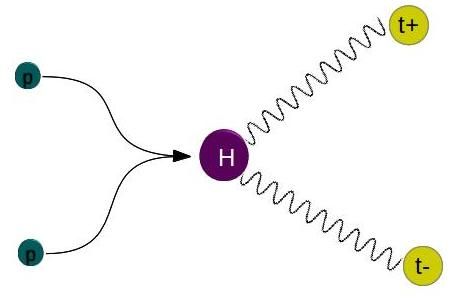
\includegraphics[scale=0.5]{Images/H1.jpg}
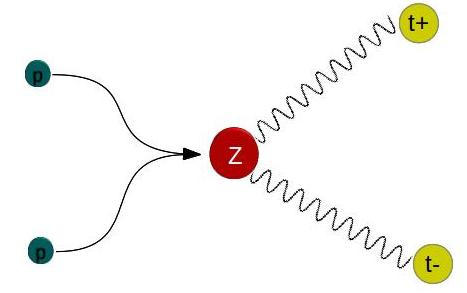
\includegraphics[scale=0.5]{Images/Zb.jpg}
\caption{The Higgs (H) and Z-boson decaying to two taus}
\label{H_decay}
\end{figure}

\item{Taus are heavy and unstable, they decay instantaneously. Their dominant decay modes involve neutrinos and the presence of these undetectable particles in their decay make it difficult to reconstruct the mass of the Higgs on an event by event basis.}
\end{itemize}

\begin{figure}
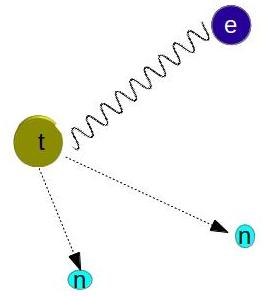
\includegraphics[scale=0.5]{Images/Te.jpg}
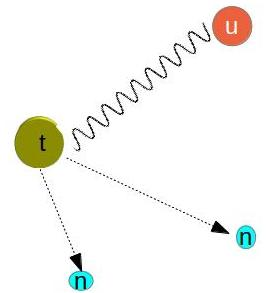
\includegraphics[scale=0.5]{Images/Tm.jpg}
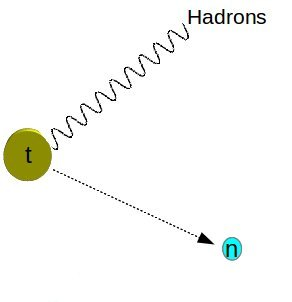
\includegraphics[scale=0.4]{Images/Th.jpg}
\caption{The tau decay to an (i) electron and 2 neutrinos, (ii) muon and 2 neutrinos, (iii) hadrons and a neutrino}
\label{Tau_decay}
\end{figure}

\subsection{A Note on the Higgs Mass}

The mass of the Higgs boson does not directly fall out of the standard model. In 2011 data collected by the CMS allowed a first thorough investigation into the existence of the SM Higgs over a wide mass range. The experiment yielded a first cut excluding the Higgs mass in the range of 127-600 GeV. This left a narrow window where a low-mass Higgs could still exist. In the region below 127 GeV the analysis showed a signal in the vicinity of 124 GeV, however, more data would be required to resolve the precise mass and reach a statistical significance of around 5$\sigma$. The LHC operation at 8 TeV in 2012 coupled with improved statistical analysis revealed an excess of events resolving to a particle with a mass of 125 GeV and this was agreed upon by the collaboration. 

\section{Machine Learning Challenge}
\label{MLC}
Both background and signal events in our dataset have the same topology,  they are tau-tau events where one tau decays into a lepton (electron or a muon) and 2 neutrinos and the other tau decays into hadrons and a neutrino. Additionally, properties of jets which originate from a high energy quark are measured by the detector.

Parent (Higgs / Non-Higgs) $\rightarrow$ $\tau^{-}\tau^{+}$ $\rightarrow$ lepton ($e^{-}$ or $\mu^{-}$) + Hadronic-tau + (Neutrinos) + Jets
 
The signal events represent collisions where the parent Higgs was created and background events represent collisions where the parent particle was not Higgs but shared the same tau-tau decay channel. The neutrinos are in parentheses to denote that their properties are not measured. The only feature pertaining to the neutrinos is the missing transverse momentum explained in Section \ref{missing}.

\subsection{The Dataset}

The signal events in the dataset have a class label 1 and background events have class label 0. The training set consists of 250,000 rows, each row denotes a collision event. The columns represent features which would serve as inputs to the classifier. The primary features are described in \ref{features}. Each row has a non-negative weight which corrects for the mismatch between the natural probability of a signal event and the probability applied by the simulator. The importance weights are not given as inputs to the classifier as the weight distribution of the signal and background events are very different and this would give away the class label immediately. The probability of a signal event in the natural world is several magnitudes lower than that of a background event. The signal and background events in the simulated dataset  are re-normalized to produce a more balanced classification problem where the ratio of signal to background events is close to 30 : 70. While the weights are not used as inputs they are used in assessing the performance of classifiers \cite{CMS:1}.

\subsection{Features}
\label{features}

The primary features in the dataset comprise of 3 measured properties of each of the detectable final-state particles and pseudo-particles. The measured properties are :

\begin{itemize}[noitemsep]
\item Pseudorapidity 
\item{Azhimuth angle} 
\item{Transverse momentum}
\end{itemize}

The final-state particles and pseudo-particles are :

\begin{enumerate}[noitemsep]
\item{Hadronic-tau} 
\item{Lepton} 
\item{Leading Jet}
\item{Sub-leading Jet}
\end{enumerate}

A full description of the physical meaning of each of the measured properties is in \ref{Pfeatures} The list of primary features, as in \cite{RM} :

\begin{enumerate}[noitemsep]
\item{\textbf{PRI$\_$tau$\_$pt} The transverse momentum $\sqrt{p_{x}^2 + p_{y}^2}$ of the hadronic tau.}
\item{\textbf{PRI$\_$tau$\_$eta} The pseudorapidity $\eta$ of the hadronic tau.}
\item{\textbf{PRI$\_$tau$\_$phi} The azhimuth angle of the hadronic tau.}
\item{\textbf{PRI$\_$lep$\_$pt} The transverse momentum $\sqrt{p_{x}^2 + p_{y}^2}$ of the lepton (the type of lepton whether electron or muon is not known).}
\item{\textbf{PRI$\_$lep$\_$eta} The pseudorapidity $\eta$ of the lepton.}
\item{\textbf{PRI$\_$lep$\_$phi} The azhimuth angle $\phi$ of the lepton.}
\item{\textbf{PRI$\_$met} The missing transverse momentum $E_{miss}^{T}$.}
\item{\textbf{PRI$\_$met$\_$sumet} The total transverse energy in the detector.}
\item{\textbf{PRI$\_$met$\_$phi} The azhimuth angle $\phi$ of the missing transverse energy.}
\item{\textbf{PRI$\_$jet$\_$num} The number of jets, either 0, 1, 2 or 3.}
\item{\textbf{PRI$\_$jet$\_$leading$\_$pt} The transverse momentum $\sqrt{p_{x}^2 + p_{y}^2}$ of the leading jet.}
\item{\textbf{PRI$\_$jet$\_$leading$\_$eta} The pseudorapidity $\eta$ of the leading jet.}
\item{\textbf{PRI$\_$jet$\_$leading$\_$phi} The azhimuth angle $\phi$ of the leading jet.}
\item{\textbf{PRI$\_$jet$\_$subleading$\_$pt} The transverse momentum $\sqrt{p_{x}^2 + p_{y}^2}$ of the sub-leading jet.}
\item{\textbf{PRI$\_$jet$\_$subleading$\_$eta} The pseudorapidity $\eta$ of the sub-leading jet.}
\item{\textbf{PRI$\_$jet$\_$subleading$\_$phi} The azhimuth angle $\phi$ of the sub-leading jet.}
\item{\textbf{PRI$\_$jet$\_$all$\_$pt} The scalar sum of the transverse momentum of all the jets of the events.}
\end{enumerate}

Apart from these there are 13 derived features, most of them are computed by operations on primary features. For example, feature \textbf{DER\_pt\_h} is the vector sum of the transverse momentum of the hadronic tau, the lepton, and the missing transverse momentum. 

\subsection{The formal problem}
\label{math}

The description in this section is based on Section 4.1 of \citep{RM}.
Let $\mathcal{D} = \{(\mathbf{x}_{1},y_{1},w_{1}),...(\mathbf{x}_{n},y_{n},w_{n}) \}$ be the sample data set provided by ATLAS,     $\mathbf{x}_{i} \in \mathbb{R}^d$ is a \textit{d}-dimensional feature vector, $\textit{y}_{i} \in \{b,s\}$ is the class label and $\textit{w}_{i} \in \mathbb{R}^{+}$ is a non-negative weight associated with each sample. Let $\mathcal{S} = \{i : y_{i} = s\}$ and $\mathcal{B} = \{i : y_{i} = b\}$ represent index sets of signal and background events respectively. Also, $n_{s} = |\mathcal{S}|$ and $n_{b} = |\mathcal{B}|$ represent the number of signal and background events in the dataset. 

It is important to clarify the role of the weights associated with each sample in the training dataset. The simulated dataset differs from the real-world dataset in the frequency with which signal events occur. The fraction $n_{s}/n_{b}$ is not reflective of the proportion of the prior class probabilities $P(y = s)/P(y = b)$, this is because $P(y = s) \ll P(y = b)$ and the true distribution of events in the dataset would yield an extremely unbalanced classification problem with $n_{s}$ significantly lower than $n_{b}$.  In order to correct for this bias, all events are weighted with importance weights reflecting their true probability of occurrence.

In each class, the quantities $N_{s}$ and $N_{b}$ are defined as, 
\begin{equation}
\sum_{i \in \mathcal{S}} w_{i} = N_{s} \hspace{5mm} 
\textrm{ and } \hspace{5mm} 
\sum_{i \in \mathcal{B}} w_{i} = N_{b} 
\label{weights}
\end{equation}

These constants have physical meaning, they are the expected total number of signal and background events during the time interval over which the data has been recorded (in the dataset used, it is the year 2012).

The objective function that the classifier is trained to optimise (described in Section \ref{ams}) depends on the \textit{unnormalized} sum of weights to make the set-up invariant to the number of simulated signal and background events.

Let $ h : \mathbb{R}^{d} \rightarrow \{b,s\} $ be an arbitrary binary classifier. The selection region $\mathcal{H} = \{\textbf{x} : h(\textbf{x}) = s\}$, $\textbf{x} \in \mathbb{R}^{d}$ is the set of points classified by $h$ as a signal, these are the \textit{predicted} positives. Let $\hat{\mathcal{H}}$ denote the index set of points that $h$ classifies as signal, $$ \hat{\mathcal{H}} = \{i : \textbf{x}_{i} \in \mathcal{H}\} = \{i : h(\textbf{x}) = s \}  $$

The quantities, 
\begin{equation} 
s = \sum_{i \in \mathcal{S}\cap \hat{\mathcal{H}}} w_{i} \hspace{5mm}
\textrm{    and    } \hspace{5mm}
b =\sum_{i \in \mathcal{B}\cap\hat{\mathcal{H}}} w_{i} 
\label{unbiased}
\end{equation} 

are unbiased estimators of the expected number of signal and background events selected by the classifier $h$ as signals. $s$ and $b$ are true positive and false positive rates.  

The binary classifier $ h : \mathbb{R}^{d} \rightarrow \{b,s\} $ calculates a discriminant value $f(\textbf{x}) \in \mathbb{R},\textbf{x} \in \mathbb{R}^{d}$ which is a score giving small values for the negative class (background) and large values for the positive class (signal). One puts a threshold of choice $\theta$, on the discriminant score and classifies all samples below the threshold as belonging to the negative class ($b$) and all samples with a score above the threshold as belonging to the positive class ($s$). 

The discriminant function $f(\textbf{x})$, also called \textit{decision function}, is evolved at the time of training and applied to test samples to reach classification decisions.

Most classifiers are optimized to improve classification accuracy on a held-out test set. The classification accuracy is the fraction of correctly classified samples belonging to all classes. Using the terminology \textit{TP} : True positives, \textit{TN} : True negatives, \textit{P} : Positives and \textit{N} : Negatives, the classification accuracy is defined as 
the fraction $\frac{\displaystyle TP + TN}{\displaystyle P + N}$. In the context of our problem a metric such as the overall classification accuracy is a weak indicator of the performance of a classifier. This is because the class distributions are skewed rather than balanced. Given that around 70\% of the samples belong to the negative class, a classifier that assigns each sample to the negative class will have an accuracy score of 70\%, but this largely ignores the strength of the classifier in classifying samples of the positive class correctly. 

In many contexts the question surrounding reliable performance measurement is tied to the problem at hand. For instance, in bioinformatics, the significance of a discovery is tied to whether the false discovery rate, defined as, $\frac{\displaystyle FP}{\displaystyle FP+TP}$ (where FP : False positive and TP : True Positive) is small enough. 

In a similar spirit, the physicists at ATLAS specify an objective function to be maximized by the classifier. It is called the \textit{Approximate Median Significance} metric. The section below elaborates on the statistical motivation for its definition.

\subsection{Approximate Median Significance (AMS) Metric}
\label{ams}

The AMS is an objective function that is applied on the set of points in a region of the feature space where an excess of signal events is expected over background. This is the \textit{selection} region $\mathcal{H}$. The selection region is defined by the value of the cut-off. For a given classifier $h$ with a discriminant function $f(\textbf{x})$ for $\textbf{x} \in \mathbb{R}^d$ and cut-off value $\theta$ the selection region is defined by, $ \mathcal{H} = \{\textbf{x} : f(\textbf{x}) > \theta \}$.

The total number of events $(n)$ in the selection region of a classifier $h$ can be partitioned into two groups :

\begin{itemize}
\item{Selected Background events : \begin{displaymath} b =\sum_{i \in \mathcal{B}\cap\hat{\mathcal{H}}} w_{i} \end{displaymath} Events which are predicted by the classifier to be of the positive signal class but actually belong to the negative class, a false positive.}
\item{Selected Signal events : \begin{displaymath} s =\sum_{i \in \mathcal{S}\cap\hat{\mathcal{H}}} w_{i} \end{displaymath} Events which are predicted by the classifier to be of the positive signal class and do belong to the positive signal class, a true positive.}
\end{itemize}

The objective function is derived as follows. The occurrence of background events follow a Poisson process (in any part of the feature space, even in the selection region). Over a given time period during which events are recorded, the expected number of \textit{selected} background events is $\mu_{b}$ and its variance is also $\mu_{b}$ (the mean and variance of a Poisson random variable are identical). The normalized statistic,  \begin{equation} \hat{t} = (n-\mu_{b})/\sqrt{\mu_{b}} \sim N(0,1) \label{normal}\end{equation} where $n$ is the total number of events in the selection region serves as a test statistic for detection of signal events. A fluctuation is considered sufficiently large to claim a discovery of the signal process if it exceeds $5\sigma$, i.e. if $\hat{t} > 5$ given that $\sigma = 1$ for the normalized test statistic.

All events in the selection region of a classifier are predicted positives, this simplifies the test statistic further, $n$ which is the total number of events in the selection region is essentially $s +b$, and $\mu_{b}$ which is the expected number of selected background events (false positives) can be approximated by its empirical counterpart, $b$. Substituting this in \ref{normal} gives, 

\begin{equation}
(n-\mu_{b})/\sqrt{\mu_{b}} = ( s + b - b)/\sqrt{b} = s/\sqrt{b}
\end{equation}

This is the simplified AMS metric, essentially a ratio of the true positives to false positives. The simplified AMS metric can be quite noisy as it is entirely dependent on events which a classifier deems as \textit{selected}, the predicted positives. This can be very small and can vary significantly for small changes in classifier design. In order to make the metric more robust a stable version of the AMS metric was proposed, it is given by,  

\begin{equation}
 \textrm{ $AMS_{s}$ } = \sqrt{2((s + b)ln(1 + \frac{s}{b})-s)} 
\label{AMS} 
\end{equation}
\raisetag{-.4em}

Given a classifier $h$, $AMS_{s}$ is the discovery significance metric that needs to be optimized.

\subsection{AMS and Discovery}

In the real experiment, the problem is that of discovering new phenomenon and no examples of real signal events are available. One would simply count the total number of events $\hat{n}$ in the selection region $\mathcal{H}$. The value $\hat{n}$ follows a Poisson distribution with mean $\hat{s} + \hat{b}$ where $\hat{s}$ and $\hat{b}$ are the mean number of events from signal and background processes. If $\hat{n}$ is found to be much greater than $\hat{b}$, then the null hypothesis of background only is rejected. The significance is quantified by using the $p$-value of the background only hypothesis. 

The signal events in the simulated dataset are generated using an elaborate simulator that simulates events according to the principles of the Standard Model taking into account noise and other artifacts. The machine learning goal in the dataset at hand is to maximize discovery significance given that the signal process is present \citep{RM}.  

\subsection{AMS vs. Classification metrics}
\label{performance}

We have seen how the overall classification accuracy is a weak indicator of the strength of a classifier in the presence of unbalanced classes. On the other hand, the direct optimization of the AMS metric is prone to generating classifiers that overfit the training data as the AMS metric is fully determined by the small number of events in the selection region $\mathcal{H} = \{ \textbf{x} : f(\textbf{x}) > \theta\}$.

The value of the AMS is sensitive to the choice of threshold $\theta$ (cut-off for the discriminant score $f(\textbf{x})$). An appropriate $\theta$ is chosen by selecting a percentile level $Q_{k}$ of $f(\textbf{x})$ where $k$ denotes the percent of values below $Q_{k}$. For instance, $\theta$ can be chosen as the 80th percentile of $f(\textbf{x})$, $\theta = Q_{80}$, this would imply that the  selection region $\mathcal{H}$ consists of the top $20\%$ of the values of $f(\textbf{x})$. To put it in terms of rejection threshold, this would imply a rejection threshold of $80\%$.

\begin{figure}
\hspace{-2mm}
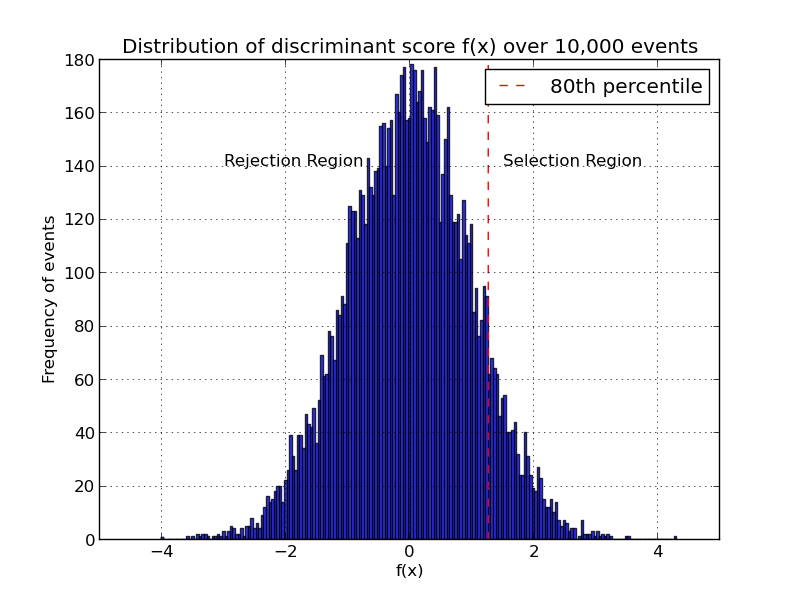
\includegraphics[scale=0.4]{Images/Selection_region.png}
\caption{This figure shows the idea of the cut-off ($\theta$) on the discriminant scores. The points to the right of $\theta$ are the predicted positives.}
\end{figure}

Below are the steps required to compute the AMS value for a classifier $h$.
\begin{enumerate}
\item Select a threshold $\theta$ for the discriminant score $f(\textbf{x})$ by choosing a percentile level $Q_{k}$.
\item Compute selected signal $s$ and background events $b$ using the importance weights provided, as in eq. \ref{unbiased}. 
\item Compute $AMS_{s}$.
\end{enumerate}

It is interesting to note the relationship between the simplified AMS metric $s/\sqrt{b}$ and the \textit{Receiver Operating Characteristic} (ROC) curve \footnote{The rather unusual name ROC emerged during World War II for the analysis of radar images. Radar operators had to decide whether a blip on the screen was an enemy target, friendly ship or just noise. Signal detection theory measures the ability of radar receiver operators to make these import distinctions. Their ability to do so was called \textit{Receiver Operating Characteristics}}.  The ROC curve illustrates the performance of a binary classifier by plotting the true positive rate (TPR = TP/P), also called \textit{sensitivity} against the false positive rate (FPR = FP/N). A fixed discriminant threshold gives a single TPR and FPR (a single point on the curve), the curve is generated by computing the TPR and FPR for different values of the discriminant threshold. Fig. \ref{roc} is an example of ROC curves for 3 different classifiers. 

\begin{figure}
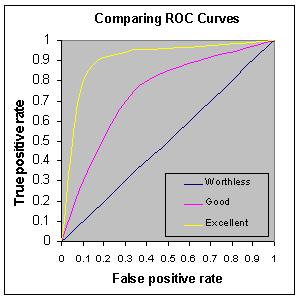
\includegraphics[scale=3]{Images/Comparing_ROC.jpg}
\caption{ROC curves for classifiers with different levels of prediction accuracy}
\label{roc}
\end{figure}

The $45^\circ$ line denotes a random classifier, which at no threshold gives a higher TPR than FPR. An ROC curve that lies above the $45^\circ$ denotes a classifier with higher than random classification accuracy of positive samples for all values of the threshold and encloses a larger area under the curve. A perfect classifier has a TPR = 1 and FPR = 0 denoting perfect accuracy. The closer the ROC curve for a classifier is to the upper left corner of the graph (1,0) the more accurate the classifier. The value on the $x$-axis, the FPR is also expressed as (1 - \textit{specificity}), where  specificity is the true negative rate (TN/N).

The slope of the tangent line to the ROC curve at a fixed threshold is the ratio $\frac{\displaystyle TPR}{\displaystyle FPR}$. This is also called the positive likelihood ratio $(LR+)$, 

\begin{equation} 
LR+ = \frac{TPR}{FPR} = \frac{sensitivity}{(1 - specificity)} 
\end{equation}

It is easy to see that this ratio (slope of the tangent line) is maximised at the extreme upper-left hand corner of the ROC curve, this is the point that gives the best trade-off between  the true positive rate and false positive rate. It is a reasonable approach in binary classification try to maximise the LR+ of a classifier in order to improve its overall classification accuracy.

Recall that the AMS metric $(s/\sqrt{b})$ is essentially the ratio of true positives to false positives in a selection region $\mathcal{H}$ specified by a cut-off threshold $\theta$. Maximizing the AMS is tantamount to maximizing the true positives and minimizing the false positives in the selection region. This is very close to the idea of maximizing the positive likelihood ratio $(LR+)$. However, there are two fundamental differences between the idea of the AMS and the ROC.

\begin{enumerate}
\item Computing the ratio of true positives to false positives in the AMS metric is tied to importance weights associated with samples in the selection region, 
\begin{displaymath}
\frac{s}{\sqrt{b}} = \frac{\sum_{i \in \mathcal{S}\cap\hat{\mathcal{H}}} w_{i}}{\sqrt{\sum_{i \in \mathcal{B}\cap\hat{\mathcal{H}}} w_{i}}}
\end{displaymath}This distorts the relationship between the likelihood ratio and AMS metric. It is possible to achieve a higher AMS metric at a point on the ROC curve where the LR+ ratio is not maximized.
\item{The area under the ROC curve, also called AUC or ROC\_AUC score integrates over all possible values of the cut-offs while the AMS considers a single point. It is computed by fixing a cut-off and ignoring all samples outside that cut-off.}
\end{enumerate}

The numerator and denominator of the LR+ ratio are rates rather than counts. The TPR = TP/P and FPR = FP/N, hence TPR/FPR = (TP/FP)*(N/P). In AMS we are dealing with counts, the actual number of true positives and false positives which are estimated as sum over importance weights. In the absence of weights the two ratios would be more homogeneous but in the presence of weights they are more de-linked. 
It is clear that optimizing the ROC curve is not the same as optimizing for the AMS. 

The \textit{precision} metric which is calculated as, $\frac{\displaystyle FP}{\displaystyle TP+ FP}$ is also closely related to the AMS metric. The precision of a classifier is (1 - False Discovery rate (FDR)) where $FDR = \frac{\displaystyle FP}{\displaystyle TP+ FP}$. In a ranked set of events (rank by value of discriminant score $f(\textbf{x})$ where the candidate signals come first), we are interested in estimating with confidence the fraction of falsely discovered events \cite{RM}. This is because highly ranked false discoveries (false positives) bring the AMS value down as they end up in the selection region. However, optimizing for precision or FDR is not an equivalent objective to the AMS as the former is a mere fraction of correct predictions and does not incorporate importance weights. 

\subsection{AMS and Balanced Classification Error}
\label{AMSbce}
A metric that closely matches the fluctuations in the AMS must incorporate the importance weights. One that is proposed by ATLAS physicists is the \textit{balanced classification error}. It is defined as, 

\begin{equation} 
R(f) = \sum_{i=1}^{n}w_{i}'\mathbb{I}\{y_{i}^{pred} \neq y_{i}^{true}\}. 
\label{bce}
\end{equation}

$\mathbb{I}$ is the indicator function. The weights $w_{i}'$ are normalized in both the signal and background classes to $N_{b}' = N_{s}' = 0.5$, that is, 

\begin{equation}
w_{i}' = w_{i}  \hspace{2mm} \times 
\begin{cases}
\dfrac{1}{2N_{s}} & \textrm{ if } i \in \mathcal{S} \\
\dfrac{1}{2N_{b}} & \textrm{ if } i \in \mathcal{B} 
\end{cases}
\end{equation}
 
A classifier is trained to minimize the balanced classification error as in eq. \ref{bce}. The AMS is then optimized with respect to a selection threshold $\theta$ in the classifier that classifies according to $sign(f(\textbf{x}) - \theta)$. Prior experiments at ATLAS suggest that the AMS is optimized at a threshold $\theta$ yielding a selection region $\mathcal{H} = \{ \textbf{x} : f(\textbf{x}) > \theta \}$ that is a small subset of the positive region $\{ \textbf{x} : f(\textbf{x}) > 0\}$ defined by the balanced classifier $sign(f(\textbf{x}))$.

It is important to re-balance the weights used in the classification error in order to penalize misclassified signals as severely as misclassified background events. Recall that the original weights $w_{i}$ for signal events are on average 300 times smaller than those for background events. %The AMS is \textbf{always} computed on unnormalized weights as in eq. \ref{weights}

\section{Decision Trees}
\label{DT}
Decision trees (DT) are predictive and non-parametric models which use supervised learning for the task of classification. Given a set of training points $\{\textbf{x}_{i},y_{i}\}$ where $\textbf{x}_{i} \in \mathbb{R}^d$ is an input feature vector and $y_{i}$ is a categorical class variable the DT learns simple rules inferred from the input features with the goal of mapping them to their correct class labels.Typically, a decision tree has a top-down flow-chart like structure, see fig. \ref{simple_tree}.

Fig. \ref{simple_tree} expresses the data in table \ref{simple_train}. 

\begin{table}[ht]
\begin{center}
\begin{tabular}{l|l|c}
$x_{1}$ & $x_{2}$ & $ x_{1} \bigoplus x_{2}$\\
\hline
0 & 0 & 0 \\
0 & 1 & 1 \\ 
1 & 0 & 1 \\
1 & 1 & 0 
\end{tabular}
\end{center}
\caption{Training data set for the binary $\bigoplus$ operator.}
\label{simple_train}
\end{table}

\begin{figure}
\hspace{-1cm}
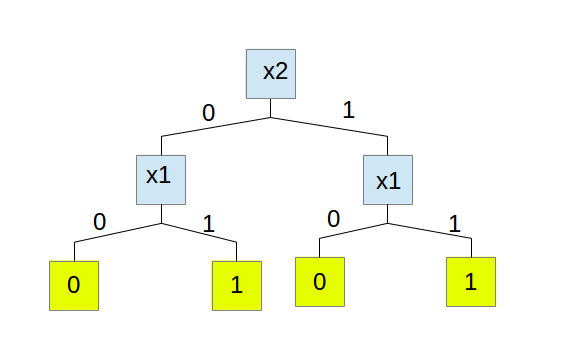
\includegraphics[scale=0.48]{Images/simple_tree.png}
\caption{Binary XOR operator training data in \ref{simple_train} expressed as a tree}
\label{simple_tree}
\end{figure}

At the top of the tree is a single \textit{source} node which at the beginning of the learning process has all the training data points. A tree starts learning by splitting the source node on the basis of a value test on a chosen input feature attribute. The value test essentially applies a threshold on the value of the chosen feature attribute and   partitions the training set. The partitions are expressed in the form of branches that emerge from the source node. This process is repeated in a recursive manner on each of the derived subsets. Fig \ref{flow_tree} illustrates the procedure of recursive partitioning. The choice of feature attribute to split on and the threshold for the value test are tied to user specified splitting criterion, this is the subject of section \ref{split}.
 

\begin{figure*}
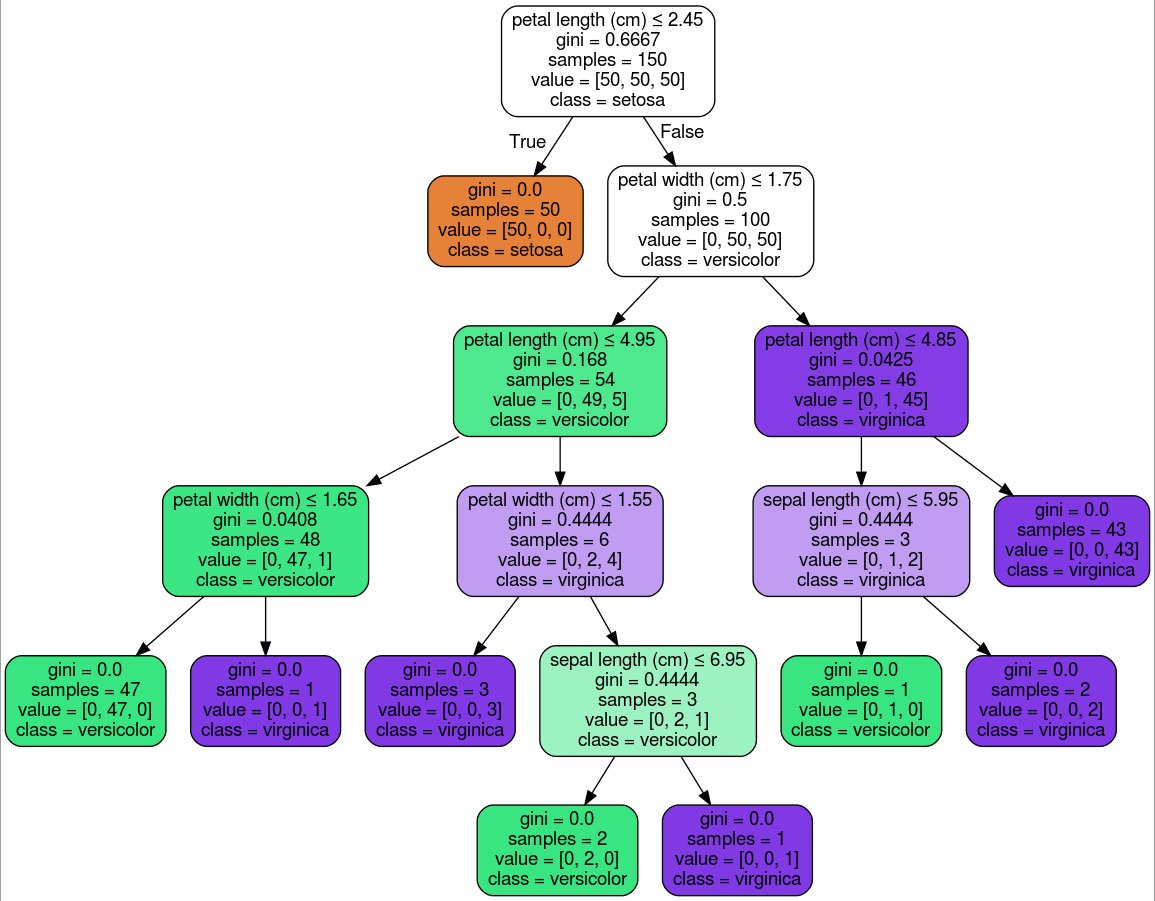
\includegraphics[scale=0.4]{Images/flow_chart.png}
\caption{Decision tree implementation on the Iris dataset based on the gini splitting critierion.}
\label{flow_tree}
\end{figure*}

A top-down recursive tree model, which by far is the most popular strategy for expressing trees has 3 main components :

\begin{enumerate}
\item{Internal nodes : Each internal node in the decision tree represents a test on an input feature.}
\item{Branches : The branching operation can be thought of as expressing a partition on the value of a input feature.}
\item{Leaf nodes : Leaf nodes are the terminal nodes of tree branches, they represent the end of the branching operation through recursive partitioning and are either labelled with a class label (when all samples in the node have the same class label) or a distribution of samples in each class.} 
\end{enumerate}

The recursive phase of the tree continues until a stopping criterion is triggered. Some of the most common stopping rules are, 

\begin{enumerate}
\item{All of the training samples in a partition belong to the same class -- in this case, the node is converted to a leaf and recursion continues on the other branches.}
\item{User specified maximum depth has been reached.}
\item{A partition has less than the minimum number of samples required for a split, this parameter can be user specified, the default value is 2.}
\item{The best splitting criterion is not greater than a certain threshold \cite{IND}.}
\end{enumerate} 

The next section describes two of the most popular splitting criterion used to incrementally grow top-down recursive trees. 

\subsection{Splitting Criterion}
\label{split}
\subsubsection{Gini index}
The gini impurity is a decision tree splitting metric used by the CART\footnote{Discussed in section \ref{CART}} algorithm. In decision trees used for classification, the gini index is used to compute the impurity of a data partition. Given a training set $S$ and a target attribute that takes on $k$ different values (classes), the gini index $\mathcal{G}$ of set $S$ is defined as,
   
\begin{align*}
\mathcal{G}(S) &= \sum_{i=1}^{k} p_{i}(1 - p_{i})  \\
&= \sum_{i=1}^k(p_{i} - p_{i}^2) \\
&= \sum_{i=1}^k p_{i} - \sum_{i=1}^k p_{i}^2 \\
 &= 1 - \sum_{i=1}^k p_{i}^{2}  
\end{align*}

where $p_{i}$ is the probability of an item chosen at random from the training set belonging to class $i$. If a subset has only 1 class, its gini index is $0$ $(=1 - 1^{2})$, such a set is a pure dataset. On the other hand if the class distribution is balanced i.e. probability of an item belonging to class $i$ is $1/k$, its gini index achieves the maximum.

The gini splitting criterion requires the computation of a gini gain $\hat{\mathcal{G}}$ for each feature $f$. 

%where $S_{j}$ is the partition induced by the value of attribute $f$ and
Let feature $f$ take on $m$ unique values in $\mathbb{R}$. For each unique value $f_{j}, j = 1,...m$ the gini gain $\hat{\mathcal{G}}(f_{j},S)$ is computed as, 

\begin{align*}
\hat{\mathcal{G}}(f_{j},S) &= \mathcal{G}(S) - \mathcal{G}(f_{j},S)  \\
&= \mathcal{G}(S) - \Bigg[ \dfrac{|S_{left}|}{|S|} \mathcal{G}(S_{left}) + \dfrac{|S_{right}|}{|S|} \mathcal{G}(S_{right}) \Bigg]
\end{align*}
 
$S_{left}$ and $S_{right}$ are the partitions resulting from splitting the set on the basis of feature value $f$. $S_{left}$ represents the set with feature value $f < f_{j}$ and $S_{right}$ represents the set with feature value $f > f_{j}$. The feature $f$ and value $f_{j}$ that maximizes the gini gain $\hat{\mathcal{G}}$ are chosen as the splitting criterion at each internal node \cite{GINI}.

\subsubsection{Entropy}

Entropy as a splitting metric is used by  ID3, C4.5 and C5.0 tree algorithms. As the name suggests it is based on the concept of entropy in information theory. The entropy of a random variable is a measure of uncertainty and is mathematically defined by Shannon as \cite{ENT}, 

\begin{equation}
H(X) = \sum_{i=1}^n P(x_{i})I(x_{i}) = - \sum_{i=1}^n P(x_{i})log_{b}P(x_{i})
\end{equation} 

where X is a discrete random variable which takes values in $\{x_{1},...,x_{n}\}$, $b$ is the base of the logarithm used, in Shannon entropy $b = 2$ to represent encoding using bits. $I(\bullet)$ is a measure of information content for $x_{i}$ and is encoded in terms of the logarithm function.

The rationale behind using the logarithm function as a measure of information content is that it is additive for independent events. If event $1$ occurs with probability $p_{1}$, $I(p1p2) = I(p1) + I(p2)$.
If event 1 can have one of $n$ equally likely outcomes and event $2$ can have one of $m$ equally likely outcomes then there are $mn$ possible outcomes of the joint event with probability $p_{1}p_{2}$.  $log_{2}(n)$ bits are needed to encode the first event and $log_{2}(m)$ bits are needed to encode the second event then $log_2{mn} = log_2(m) + log_2(n)$ bits are needed to encode both. Any function that encodes information content should preserve this additivity, hence the choice is logarithmic .i.e. $I(p) = log(1/p)$ \cite{ENT}.
  
Information gain under the entropy metric is defined as, 

\begin{equation}
IG(T,f) = H(T) - H(T|f)
\end{equation}

where T is a set of training samples, $H$ is the entropy of the parent training set and $H(T|f)$ can be thought of as the weighted entropy of the left and right partition sets induced by a partition on the feature value of $f$. Let $f$ take $m$ unique values in $\mathbb{R}.$ For each unique value $f_{j}, j = 1,...m$ the information gain $IG(T,f_{j})$ is computed as,

\begin{equation}
IG(T,f_{j}) = H(T) - \Bigg[ \dfrac{|T_{left}|}{|T|} H(T_{left}) + \dfrac{|T_{right}|}{|T|} H(T_{right}) \Bigg]
\end{equation} 

where $H(T) = -\sum_{i=1}^{k}p_{i}log_{2}p_{i}$ in the presence of $k$ classes and $p_{i}$ is the probability of a sample chosen at random belonging to class $i$. 

Intuitively, both the gini gain and entropy splitting criteria can be thought of as metrics that measure the reduction in impurity from a split and select a split that maximizes this reduction. 

\subsection{Mathematical Formulation}

Given input feature vectors $\{\textbf{x}_{i}\} \in \mathbb{R}^d$ and a target variable $y_{i} \in \{0,1\}$, a DT recursively partitions the training set at each node. 

Without loss of generality, let the data at node $q$ be represented by $Q$. The DT considers for each candidate split $\phi = (f,f_{j})$ where $f$ is a feature and $f_{j}$ a threshold, partitions of the data $Q$ into left and and right sets $Q_{l}$ and $Q_{r}$ such that,

\begin{gather*}
Q_{l}(\phi) = \{\textbf{x}_{i} \in Q : \textbf{x}_{i} \leqslant f_{j}\} \\
Q_{r}(\phi) = \{\textbf{x}_{i} \in Q : \textbf{x}_{i}> f_{j}\}
\end{gather*}

The impurity denoted by $\mathcal{E}(\bullet)$ at node $q$ is computed for all valid candidate splits $\phi$ on $Q$ as, 

\begin{equation}
\mathcal{S}(Q,\phi) = \dfrac{Q_{l}}{Q}\mathcal{E}(Q_{l}(\phi)) + \dfrac{Q_{r}}{Q}\mathcal{E}(Q_{r}(\phi)) 
\end{equation}

The candidate set $\phi$ that minimizes the sum of impurities of left and right sets is chosen as the parameter for the split.

\begin{equation}
\phi = \argmin_{\phi}\mathcal{S}(Q,\phi)
\end{equation}

These steps are applied recursively for sets $Q_{l}$ and $Q_{r}$ to grow the tree until one of the stopping criteria are triggered or all the samples in the node belong to the same class. 
\cite{MDT}

\subsection{Decision Trees as classifiers}

\subsubsection{Advantages}
Non-parametric DTs have several advantages that make it a strong choice for classification problems in both linear and non-linear settings. Some of the main advantages of DTs are summarised below, 

\begin{enumerate}
\item{Trees have a visual quality, it is possible to visualize a tree model with all the internal and leaf nodes along with the decision rules at each level.}
\item{Tree algorithms require little or no data processing. Models like SVMs on the other hand require one or two steps of data processing like scaling of features and normalization.}
\item{Trees can be used for classification and regression tasks with very little modification.}
\item{DTs are fast to train as opposed to algorithms like neural nets and SVMs, they have the advantage of speed and scalability. The cost of using the tree is logarithmic in the number of data points used to train the tree.}
\item{As opposed to neural nets which are more opaque the classification rules of a decision tree are immediately interpretable.}
\item{Tree algorithms have several inbuilt approaches for dealing with missing values, for instance in C4.5 samples with missing values are distributed to leaf nodes but with diminished weights proportional to the number of instances in each leaf node.}
\item{Several optimized algorithms in a wide variety of languages are available for tree learning like SHARK \cite{SHARK} and MLPACK \cite{MLPACK} for C++ and \texttt{sklearn} \cite{SKLEARN} for Python.}
\end{enumerate}

\subsection{Disadvantages}

\begin{enumerate}
\item{The fact that trees can be grown parameter free leads to a high chance that trees can end up being over-complex and deep. They have a tendency to over fit the training data and do not generalize well to test data. Parametric trees on the other hand which have user specified parameters that control for maximum depth and minimum samples at each leaf node can alleviate this problem.}
\item{Trees can have a high variance in their output, small perturbations in the input can give different solutions. A popular choice is to use DTs within an ensemble of many different classifiers.} 
\item{Greedy algorithms which are one of the most popular tree learning strategies do not guarantee global optimum, whereas algorithms like SVMs which entail maximization or minimization of a convex objective guarantee global optimum.}
\item{DTs do not immediately give probabilistic outputs and need to be modified or post-processed for soft classification problems which rely on a probabilistic output.}
\item{In the presence of skewed class distributions DTs can create biased trees. In this case one might have to balance the dataset prior to fitting.}
\end{enumerate}

\section{CART Algorithm}
\label{CART}
CART stands for \textit{Classification and Regression trees} and was developed by Brieman et al (1984). A CART tree is essentially a binary decision tree which is constructed by splitting the source node (which contains the full training set) recursively until a stopping criteria is triggered or until a node is homogeneous .i.e. all samples belong to the same class.  

The CART algorithm employs an exhaustive process to choose splits. It chooses the best split among all possible splits to divide each internal node. Since CART makes the locally optimal choice at each stage it is a greedy algorithm.

Below is the pseudocode for the CART algorithm implemented in \texttt{sklearn.DecisionTreeClassifier}

\begin{algorithm}
\caption{CART Algorithm for binary classes}
\begin{algorithmic}[1]
\STATE Start at root node $T$
\IF{All samples belong to class : 0} 
\STATE Return $T$
\ELSIF{All samples belong to class : 1} 
\STATE Return $T$
\ELSE 
\STATE Start Recursion 
\WHILE {T is non-empty}
\STATE Check for stopping criteria
\STATE Compute impurity $\mathcal{S}(T)$ for all possible $\phi$
\STATE Select best $\phi$
\STATE Create new nodes $\Rightarrow$ $T_{l}$ and $T_{r}$
\STATE Go back to step 9 for all new nodes
\ENDWHILE
\STATE End Recursion
\ENDIF 
\end{algorithmic}
\end{algorithm}

The popularity of the CART methodology can be attributed to several practical factors, they are :

\begin{enumerate}[label=(\roman*)]
\item{CART can handle both numerical and categorical features.}
\item{The method is robust to outliers, the splitting algorithm isolates outliers by branching them out to individual nodes.}
\item{The method is equipped to handle missing values of features by considering surrogates (values of other features that can replace the missing feature). This gives reasonable performance however one has to carefully account for this behaviour in problems where applying surrogates for missing features is not an option.}
\item{The structure of the final tree is invariant to monotone transformation  of features.}
\item{CART is computationally inexpensive, the time complexity of building an unpruned decision tree considering all features at each node is $O(mnlogn)$ where $m$ is the number of features and $n$ is the number of training samples.}
\end{enumerate}

\section{Probability calibration}
\label{prob_calib}
In several supervised classification domains there is a need to provide viable probability estimates for class membership. In CART, ID3 and C4.5, three of most popular tree learning algorithms the probability score for a test sample  is by default the raw training frequency $p = k/n$. Here, $k$ is the number of positive training samples in the leaf the test sample ends up in and $n$ is the total number of samples belonging to all classes in that leaf. A simple demonstration of this is in fig. \ref{prob_freq_draw}. 
In the simple univariate feature tree, all test samples end up either in leaf $L$ or leaf $R$. Here the predicted probability associated with each test sample that ends up leaf $L$ or $R$ is depicted in table \ref{prob_default}. 

These training frequencies are not good estimators of conditional probability estimates due to two reasons, 

\begin{enumerate}
\item{Bias : DTs based on the entropy splitting criterion try to make leaves homogeneous, hence, the class frequencies of leaves cluster around 0 and 1. This overestimates class probabilities and are not a good indicator of class membership in soft classification models where decisions are made based on probability estimates.}
\item{Variance : For nodes with a small number of training samples, observed frequencies are not reliable. The model does not incorporate the density of a leaf node in constructing probability estimates. Density of a leaf node refers to the number of samples that end up in it after running through the decision rules top-down. A high number of samples in a leaf node increases the confidence of the raw probability estimates derived from it. For example, the model assigns test samples ending up in leaf A with a class distribution of [50,100] the identical probability of 0.33 (of belonging to the former class), as to a test sample ending up in leaf node with a distribution [1,2].}
\end{enumerate}

\begin{figure}
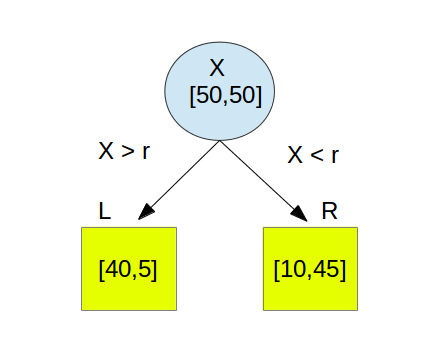
\includegraphics[scale=0.5]{Images/prob_freq.png}
\caption{Class frequencies in terminal nodes}
\label{prob_freq_draw}
\end{figure}

\begin{table}
\begin{tabular}{lll}
Terminal node identity & $P(y_{i} = 0)$ & $P(y_{i} = 1)$ \\
\toprule
L & 8/9 & 1/9 \\
R & 2/11 & 9/11 \\ 
\end{tabular}
\caption{Default probabilities assigned by CART, ID3, and C4.5 for the tree depicted in fig. \ref{prob_freq_draw}}
\label{prob_default}
\end{table}

Provost and Domingos \cite{PD} suggest a way of improving the raw probability estimates given by tree algorithms, the basic idea is to make these estimates smoother. The motive is to make them less extreme and for this they use the Laplace correction method. For a 2-class problem this would replace training frequency $p = k/n$ by 
$p' = \frac{\displaystyle k + 1}{\displaystyle n +2}$ where $k$ is the number of positive training samples in a leaf and $n$ is the total number of training samples in a leaf. The Laplace correction method adjusts probability distributions to  cluster around 0.5, this is reasonable in problems with balanced class distributions. However, in problems with unbalanced class distribution like the Higgs dataset where the ratio of signal to background is 30:70, this would lead to distorted probability measures. 

Another approach suggested in \cite{CAL} is to consider the overall probability estimate of the positive class .i.e. the $base$ rate $b$. The conditional probability estimate is smoothed towards the corresponding unconditional probability estimate given by $b$. This idea borrows from the Bayesian perspective of probability. The probability estimate $p = k/n$ is replaced by $p' = \frac{\displaystyle k + b.m}{\displaystyle n + m}$ where $b$ is the base rate and $m$ is a parameter that controls how much the training frequencies are shifted towards the base rate. This smoothing method is called $m-estimation$. It is suggested in \cite{CAL} that choosing $m$ such that $bm = 10$ ensures that leaves with $k \leqslant 10$ are given low credence. It turns out that the actual value of $m$ is unimportant and the effect of smoothing by $m$ is very similar for a wide range of $m$ values.   

\section{Learning Pipeline}

This section describes the series of steps taken to optimize the decision tree model implemented by the \texttt{sklearn.DecisionTreeClassifier} which uses an optimized version of the CART algorithm.
 
\label{learning_pipe}

\subsection{Dataset and Missing values}

The entire dataset has 250,000 rows many of which have missing values. In this analysis we focus on rows which have no missing values in any of the features and hence condense the training set by dropping rows with any missing values. The final size of the condensed dataset with no missing values is 68114. We then split this dataset into training set (TRAIN) and test set (TEST) by uniform random selection with each data point equally likely to fall into either the TRAIN or TEST set. The respective proportions of the training and test set are 75\% and 25\%. The test set is not used for cross-validation. TRAIN set is repetitively shuffled and split into 2 parts one of which is used for training and the other for validation. In a $k$-fold cross validation the shuffle split procedure is conducted $k$ times and mean scores of $k$ iterations are persisted as final scores. The procedure is described in more detail in the algorithm summarised in \ref{tree_tuning}.

\begin{figure*}
\hspace{-2cm}
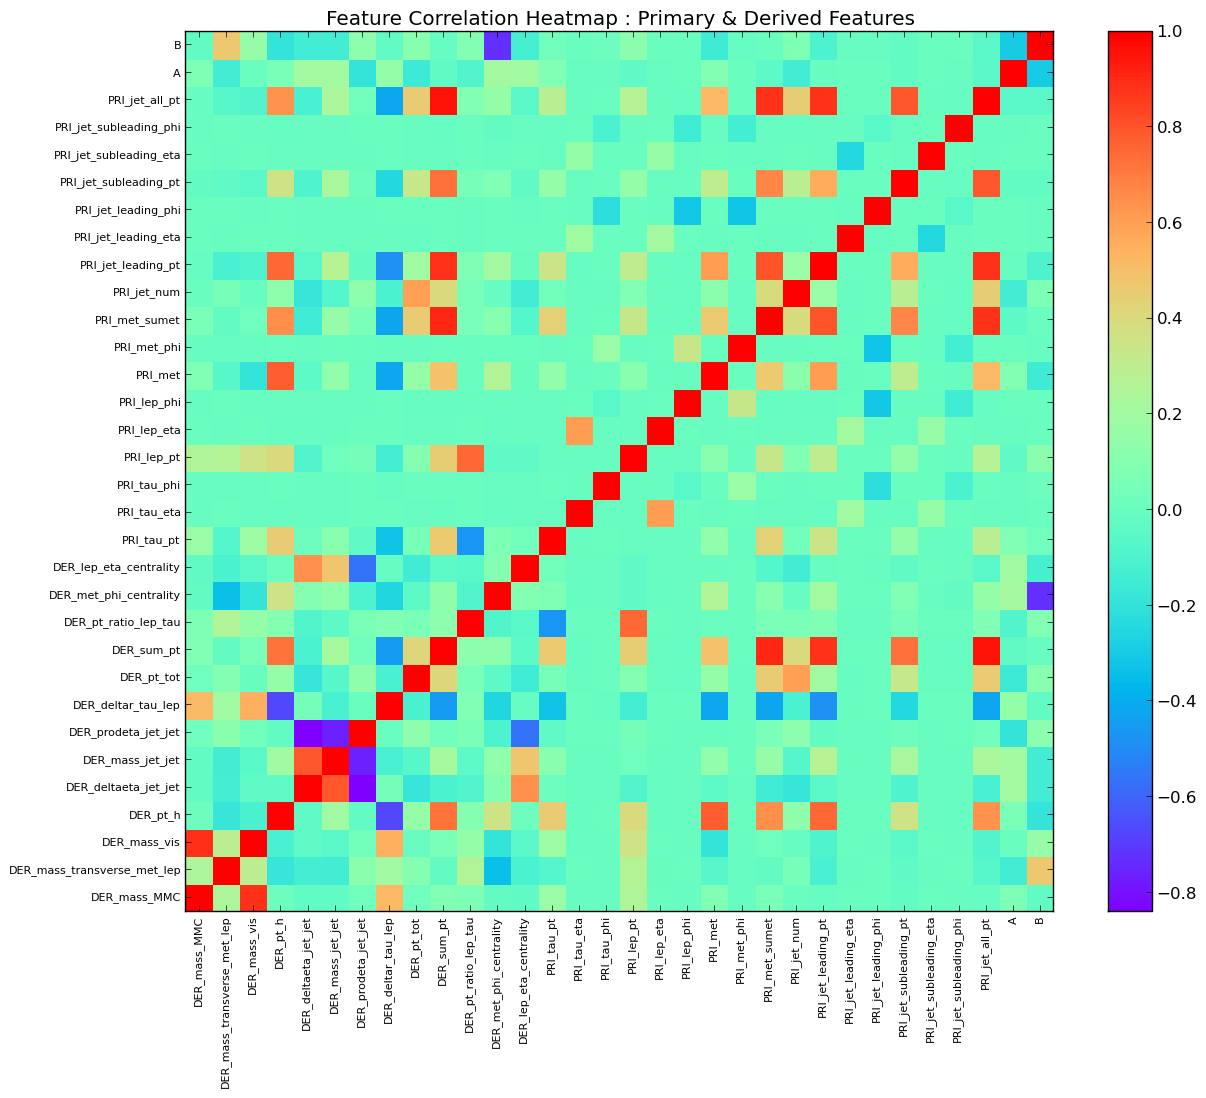
\includegraphics[scale=0.6]{Images/DERFeaturesHeatMap.png}
\caption{Feature Correlation map showing the strength of correlation between different features. It is a symmetric display with 1s on the diagonal showing correlation of a feature with itself. The features that had correlation coefficient values $|c| > 0.8$ with other features were dropped. From a group of correlated features only the one with the highest point bi-serial correlation was retained.}
\label{ff}
\end{figure*}

\subsection{Feature Selection and pruning}
The feature correlation map is depicted in fig. \ref{ff}, it shows the strength of correlation between features across both classes. 

Features that are strongly correlated with other features represent low discriminating power and can be removed without much information loss. Redundant features were identified on the basis of the strength of their correlation with other features and dropped from the dataset. We will go on to show how an optimally fitted tree that uses all features is qualitatively similar to the one that uses fewer redundant features. 

Since the class variable is dichotomous, $y_{i} \in \{0,1\} \forall i$, the feature vs. class correlation is computed using the point-biserial correlation. This is mathematically equivalent to the Pearson correlation for computing correlations between one continuous and one dichotomous variable. The point-biserial correlation was computed between each feature and the binary class variable. It is computed as, 

\begin{equation}
r_{pb} = \dfrac{M_{1} - M_{0}}{s_{n}}\sqrt{\dfrac{n_{1}n_{0}}{n^2}}
\end{equation}

where $M_{0}$ and $M_{1}$ are the mean values of the feature for the background and signal class. $s_{n}$ is the inter-class standard deviation of the feature, $n_{0}$ and $n_{1}$ represent the count of samples in the background and signal class and $n$ is the overall count. From figure \ref{biserial} it is apparent that the derived features showed higher correlation with the class label than the primary features \ref{features}. 
 
\begin{figure*}
\hspace{1.8cm}
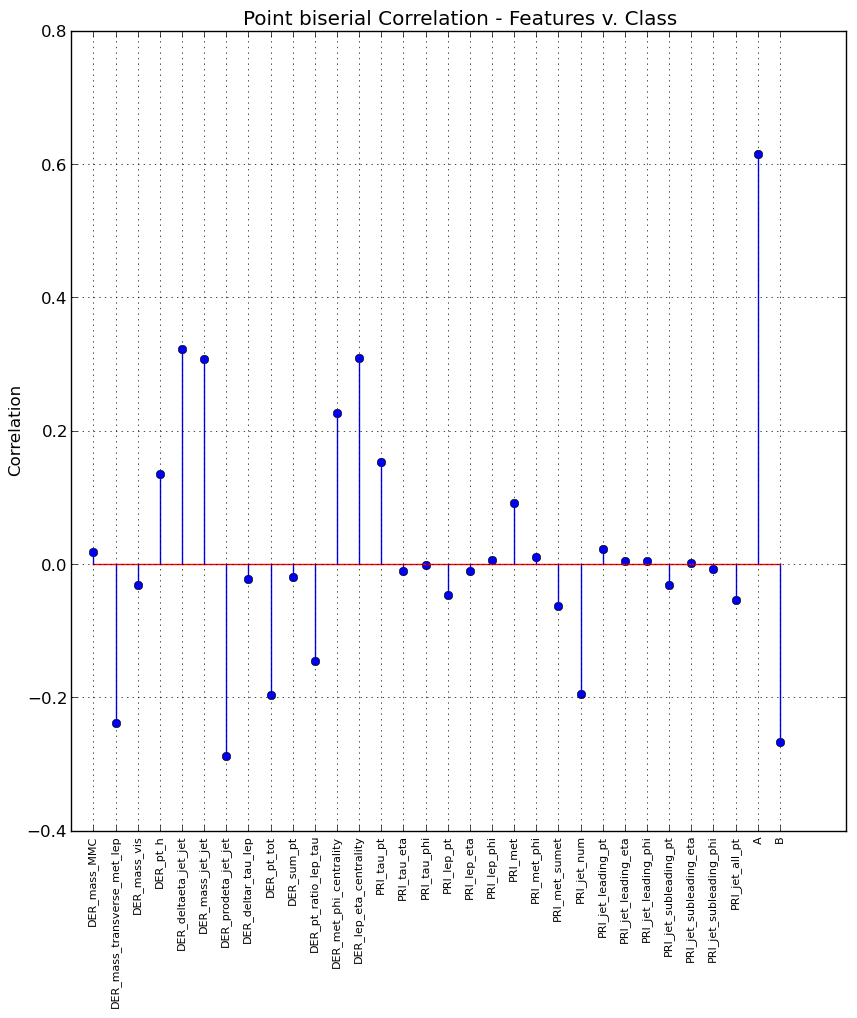
\includegraphics[scale=0.6]{Images/BiSerialCorr.png}
\caption{The figure shows the strength of correlation of derived features (DER\_$*$) over the primary features (PRI\_$*$). Derived jet features showed higher correlation and analytically derived feature A and B showed higher correlation to any of the primary features.}
\label{biserial}
\end{figure*}

Visual examination of feature distributions of signal and background gave some insight on the discriminating power of features. The derived features with higher point bi-serial correlation relative to other features were:

\begin{enumerate}[noitemsep]
\item{DER\_deltaeta\_jet\_jet}
\item{DER\_mass\_jet\_jet}
\item{DER\_prodeta\_jet\_jet}
\end{enumerate} 

Feature $A$ (also called $CakeA$) was a feature proposed by by Dr. Christopher Lester at the Cavendish Laboratory. It is computed analytically based on primary momenta of the decayed particles and rely on the calculation of a likelihood function from first principles for the event to be a signal.

It showed a high point bi-serial correlation with the class variable as can be seen in \ref{biserial} and its distribution by class is shown in \ref{dists_1}.

\begin{figure*}
\hspace{-0.9cm}
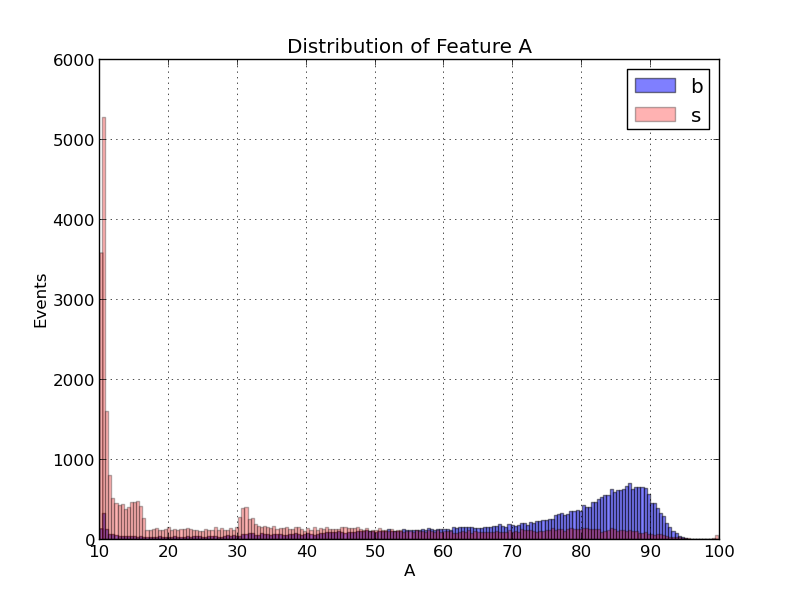
\includegraphics[scale=0.5]{Images/A_dist.png}
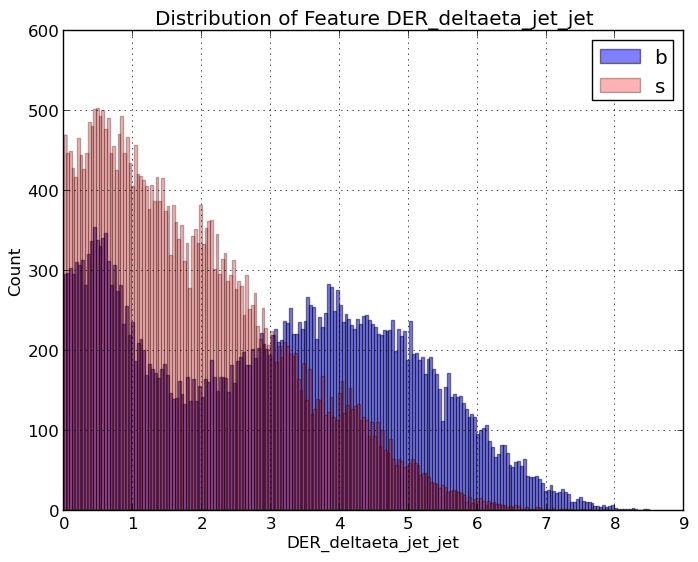
\includegraphics[scale=0.5]{Images/DER_deltaeta_jet_jet_Hist.png}
\caption{Distribution of Features by class breakdown}
\label{dists_1}
\end{figure*}

\begin{figure*}
\hspace{-0.5cm}
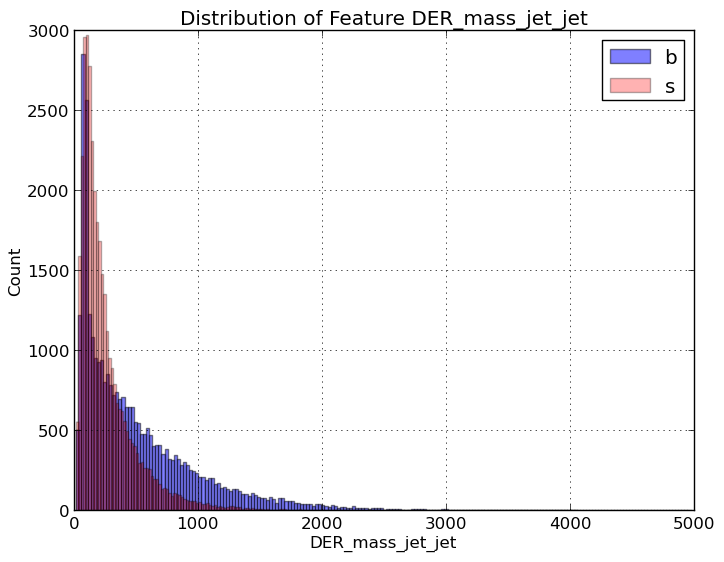
\includegraphics[scale=0.5]{Images/DER_mass_jet_jet_Hist.png}
\hspace{4mm}
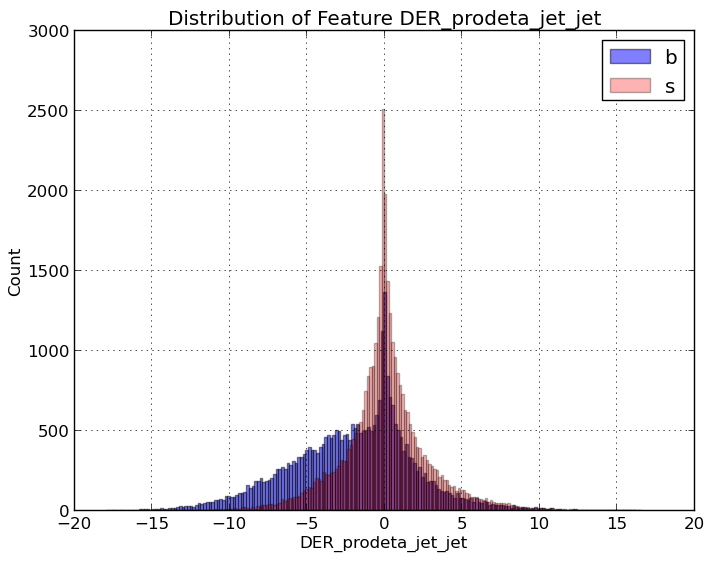
\includegraphics[scale=0.5]{Images/DER_prodeta_jet_jet_Hist.png}
\caption{Distribution of Features by class breakdown}
\label{dists_2}
\end{figure*}


%Feature $B$ ....
%Moreover $\phi$ (azhimuth angle) features were dropped as ....

\section{Hyper-parameter tuning}
In this section we describe the steps taken to optimize parameters of the decision tree. A decision tree has five main parameters that govern its design, these are :

\begin{enumerate}
\item{\textbf{Splitting criterion} : In the \texttt{sklearn.DecisionTreeClassifier} implementation we are allowed to choose between the $gini$ or $entropy$ splitting criteria.}
\item{\textbf{Max features} : This parameter controls the number of features the tree considers as a splitting choice at each internal node.}
\item{\textbf{Max depth} : This parameter acts as a stopping rule, if a branch reaches the max depth value it converts the node into a leaf even if all the samples do not belong to the same class. All nodes are expanded until either all leaves are pure or max depth value is reached.}
\item{\textbf{Minimum samples in each leaf} : This parameter controls the minimum samples that are required to be at a leaf node. If a node has less than the minimum number of samples required, it converts itself into a leaf node.}
\item{\textbf{Minimum samples split} : This parameter controls the minimum number of samples required to split an internal node. The default value for this parameter is 2.}
\end{enumerate}

Intuitively, these parameters control in different ways the growth of a decision tree by pruning and help avoid over-fitting the tree structure to the training data. 

These parameters were optimized through a grid search with 3-fold cross-validation by choosing appropriate ranges for each of the parameters and computing three different metrics :

\begin{itemize}
\item {\textbf{ROC AUC score} : This metric computes the area under the ROC curve (described in section \ref{performance}). The true positive rate and false positive rates are computed for the positive signal class.} 
\item {\textbf{Balanced Classification error} : This metric computes the misclassification score weighted by sample weights, it is defined as, 

\begin{equation} 
R(f) = \sum_{i=1}^{n}w_{i}'\mathbb{I}\{y_{pred} \neq y_{true}\}. 
\end{equation}
where $y_{pred}$ is the class label predicted by the classifier and $y_{true}$ is the true class label.
 
\begin{equation}
w_{i}' = w_{i}  \hspace{2mm} \times 
\begin{cases}
\dfrac{1}{2N_{s}} & \textrm{ if } i \in \mathcal{S} \\
\dfrac{1}{2N_{b}} & \textrm{ if } i \in \mathcal{B} 
\end{cases}
\end{equation}}
\item {\textbf{AMS Train} : AMS score as given by eq. \ref{AMSc} computed on the test data.}

The AMS can tend to be very noisy as it is sensitive to the choice of threshold $\theta$ which defines the selection region, hence we compute the AMS score over a range of thresholds $\theta$ and consider the mean value over the range. We consider for $\theta$ percentile thresholds $Q_{k}$ where $k$ ranges from $78$ to $88$. The AMS score computed is given by the equation, 

\begin{equation}
\textrm{ $AMS_{s}$ } = \sqrt{2((s + b)ln(1 + \frac{s}{b})-s)} 
\label{AMSc} 
\end{equation}
\end{itemize}

\begin{algorithm}
\caption{Tree Param Tuning}
\begin{algorithmic}[1]
\STATE Get ranges for all $m$ parameters $p_{i}, i = 1...m$ to be tuned
\STATE $|p_{i}| \leftarrow$ number of choices for parameter $i$
\STATE Compute parameter grid $G$ by enumerating $|p_{1}| \times ...\times |p_{m}|$ parameter combinations.
\FORALL {param combinations $c \in G$}
\STATE Set count = 0
\REPEAT 
\STATE Split supervised training set randomly into learn set L and validate set V  
\STATE Fit CART Tree Algorithm on L 
\STATE Apply Fitted Tree (T) to dataset V
\STATE Compute $r \leftarrow$ ROC AUC
\STATE Compute $b \leftarrow$ Balanced classification error
\STATE Compute $ams \leftarrow$ AMS
\STATE Increment count by 1
\UNTIL {count = 3}
\STATE Compute mean values from 3 iterations $r_{mean}$, $b_{mean}$ and $ams_{mean}$ 
\STATE Persist \_mean\_scores $\leftarrow (c,r_{mean},b_{mean},ams_{mean})$ 
\ENDFOR
\RETURN {\_mean\_scores}
\end{algorithmic}
\label{tree_tuning}
\end{algorithm}

\section{Results}
\label{results}

\begin{algorithm}
\caption{Learning Pipeline}
\begin{algorithmic}[1]
\STATE \textbf{Load} data from disk 
\STATE \textbf{Pre-process} data  \\
\qquad Drop missing values \\
\qquad Drop correlated features \\
\qquad Split data into training set -- TRAIN and test set -- TEST 
\STATE \textbf{Compute} baseline performance for \texttt{sklearn.DecisionTreeClassifier} trained on TRAIN and tested on TEST
\STATE $metrics$ $\leftarrow$ list of metrics to optimize  
\STATE \textbf{Start} Optimization \\
\FORALL {$m \in metrics $} 
\STATE \quad  \textbf{Run} Tree Parameter Tuning Algorithm on TRAIN \\
\qquad $\hookrightarrow$ Retrieve best parameters for metric $m$ \\  
\ENDFOR
\STATE \textbf{Finish} Optimization 
\STATE \textbf{Fit} CART tree on TRAIN with optimized parameters
\STATE \textbf{Calibrate} conditional probability estimates using leaf training frequency model
\STATE \textbf{Calibrate} conditional probability estimates using $b$ and $m$
\STATE \textbf{Compute} AMS over a range of thresholds $\theta$ 
\end{algorithmic}
\end{algorithm}
\subsection{Baseline Decision Tree}
\label{base}

The baseline performance of the decision tree classifier implemented in \texttt{sklearn} with default parameters is summarised below for two splitting criterion : Gini and Entropy.

\begin{table}
\centering
\begin{tabular}{l|l}
Parameter & Default Value \\
\toprule
Max depth & None \\
Max features & All\\
Min samples split & 2\\
Min samples leaf & 1\\
class weight & auto\\
\end{tabular}
\caption{The default parameter values used to fit a CART decision tree on the training set.}
\end{table}


All features are considered at each split, the tree grows until all terminal nodes get converted to leaves by triggering the stopping criteria. The minimum number of samples at each leaf is 1 and the minimum number to qualify for a split is 2. The class weight is inferred and is proportional to the class frequencies in the training set.

\begin{figure}
\hspace{-1.5cm}
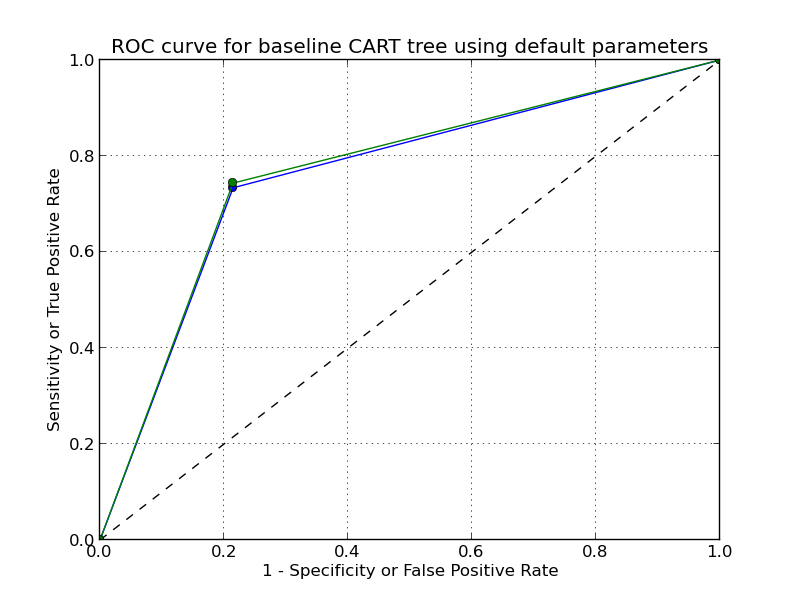
\includegraphics[scale=0.5]{Images/baseline_DT_ROC.png}
\caption{ROC curves for baseline CART trees based on TEST set}
\label{base_roc}
\end{figure}

A CART tree is fitted on the TRAIN set and performance metrics are computed on the TEST set. Since there is no parameter tuning no cross-validation is conducted.

The figure \ref{base_roc} shows the ROC performance of the baseline DT classifier applied on the TEST dataset. 

\begin{table}
\centering
\begin{tabular}{l|l|l}
Metric & Score (Gini) & Score (Entropy)\\
\toprule
ROC & 0.734 & 0.748\\
Precision & 0.75 & 0.76 \\
Recall & 0.74 & 0.75\\
\pbox{10cm}{Balanced \\Classification Error} & 26\% & 25\%\\
AMS &  1.83 & 1.84\\
\end{tabular}
\caption{Performance scores of the baseline classifier}
\end{table}


The two baseline classifiers based on the Gini and Entropy criteria are qualitatively very similar when fitted using the default parameters. The next section discusses the results of parameter tuning on the baseline decision tree. 

\subsection{Parametric decision tree}
\label{param}

The baseline CART tree parameters are optimized using a grid search with 3-fold cross-validation. The procedure is described in \ref{tree_tuning}. Overall, 1287 (429 x 3) fits were performed i.e. 3 iterations per parameter combination over 429 combinations. 

The result of the grid search in the parameter space is summarised in the table \ref{param_tree}, each column contains the best parameter choices optimized by the metric in the header row. $R(f)$ stands for balanced classification error.  

\begin{table}[ht]
\begin{tabular}{c|l|l}
Optimized Criteria & ROC\_AUC & R($f$) \\
\toprule
Max features & All & 10\\
\midrule
Max depth & 50 & None\\
\midrule
Min samples leaf & 150 & 150 \\
\midrule
Min samples split & 200 & 40\\
\midrule
Splitting Criteria & Gini & Entropy\\ 
\end{tabular}
\caption{Optimum parameters for CART tree}
\label{param_tree}
\end{table}

\begin{figure}
\hspace{-0.5cm}
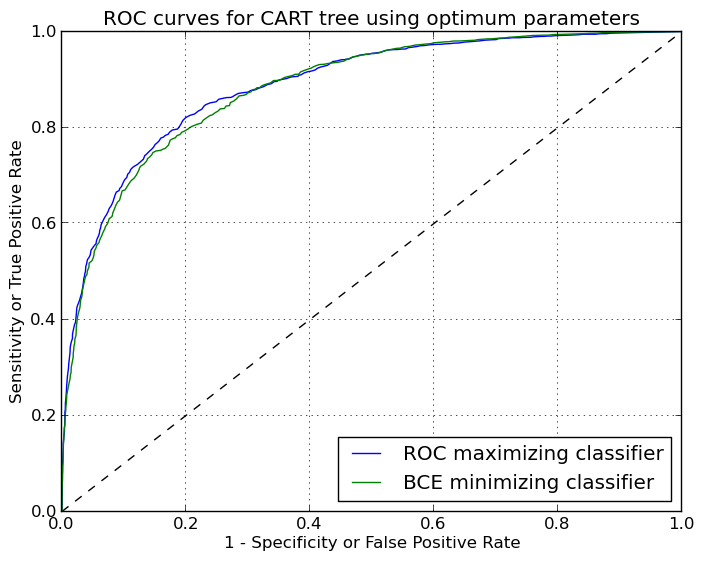
\includegraphics[scale=0.5]{Images/ROC_Optimum.png}
\caption{ROC curves for the optimized parameters}
\label{ROC_optimum}
\end{figure}

The ROC curve for the two sets of optimized parameters is shown in \ref{ROC_optimum}. As a result of the parameter tuning, the AMS has gone up by $\sim$0.7 when optimized for the balanced classification error and by $\sim$1.5 when using parameters for the ROC optimized classifier.  


The plots in \ref{param_iterate_roc} and \ref{param_iterate_bce} depict the distribution of the score metric by fixing one parameter and allowing the others to vary according to the values in the grid. We observe that the best score can be achieved at more than one combination of parameters. The grid search exercise helps to eliminate parameter choices which give lower than mean scores. We select the parameter combination which gives the highest ROC and lowest $R(f)$ score to compute the AMS metric. 

\begin{figure*}
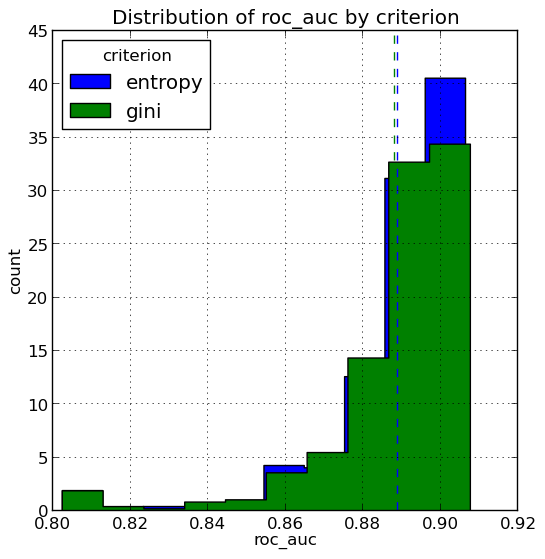
\includegraphics[scale=0.5]{Images/roc_auc_criterion.png}
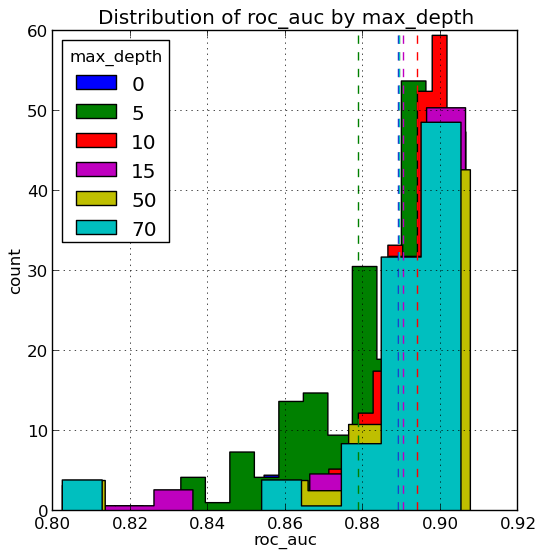
\includegraphics[scale=0.5]{Images/roc_auc_max_depth.png}
%\end{figure*}
%\begin{figure*}
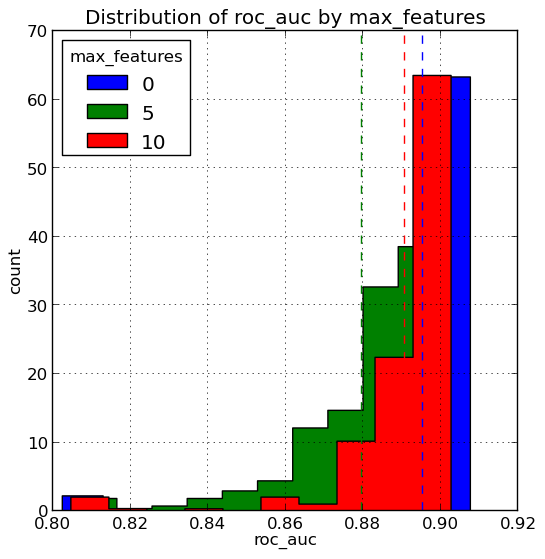
\includegraphics[scale=0.5]{Images/roc_auc_max_features.png}
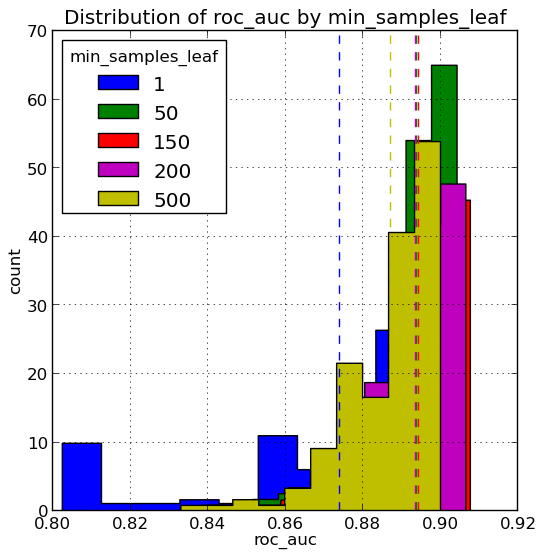
\includegraphics[scale=0.5]{Images/roc_auc_min_samples_leaf.png}
%\end{figure*}
%\begin{figure*}
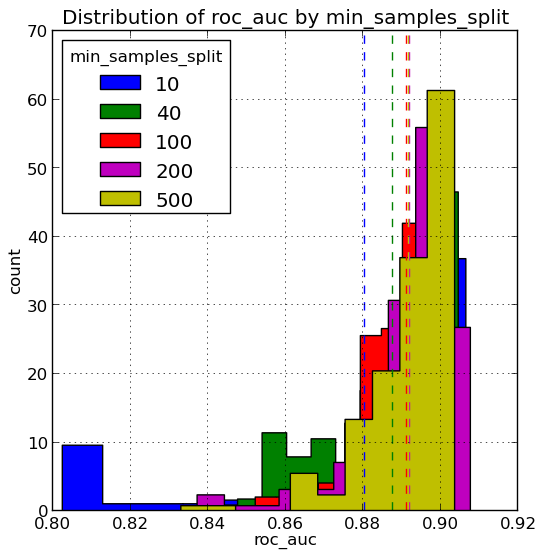
\includegraphics[scale=0.5]{Images/roc_auc_min_samples_split.png}
\caption{Scores by parameter values}
\label{param_iterate_roc}
\end{figure*}

\begin{figure*}
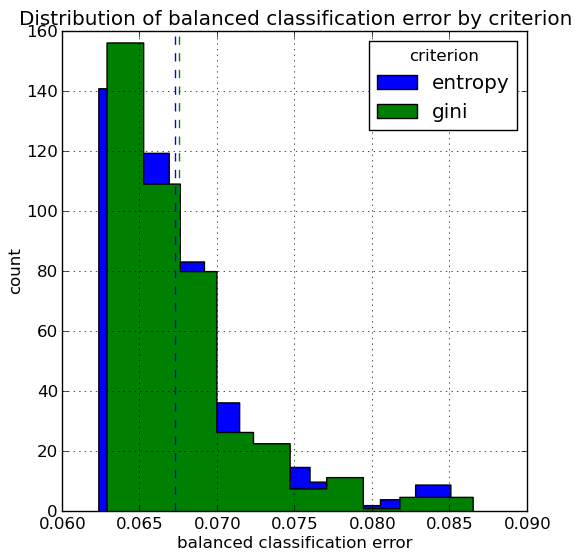
\includegraphics[scale=0.5]{Images/balanced_classification_error_criterion.png}
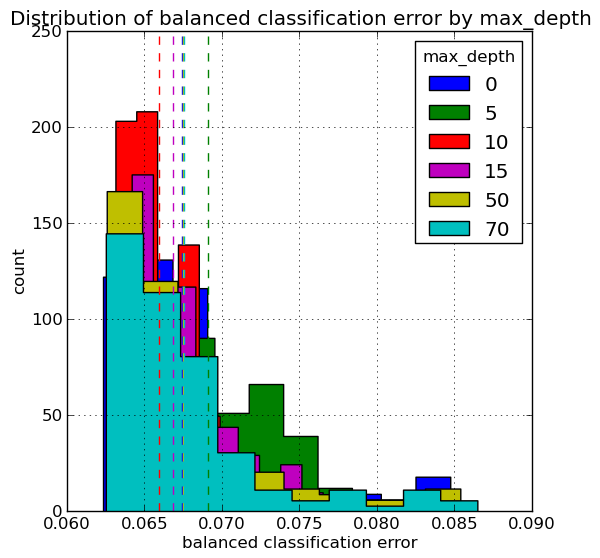
\includegraphics[scale=0.5]{Images/balanced_classification_error_max_depth.png}
%\end{figure*}
%\begin{figure*}
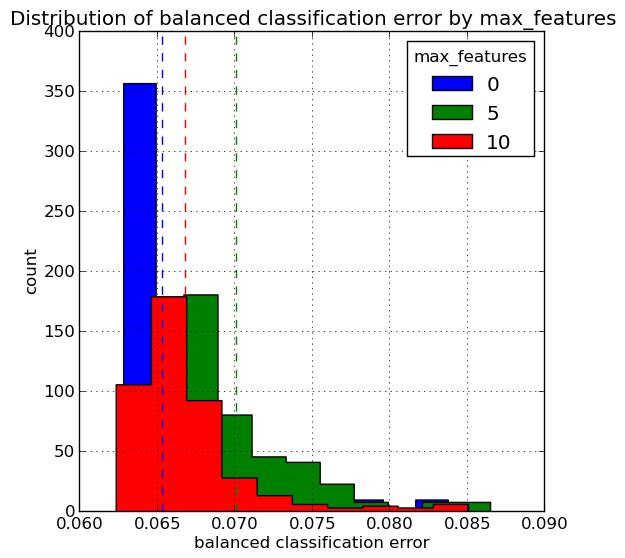
\includegraphics[scale=0.5]{Images/balanced_classification_error_max_features.png}
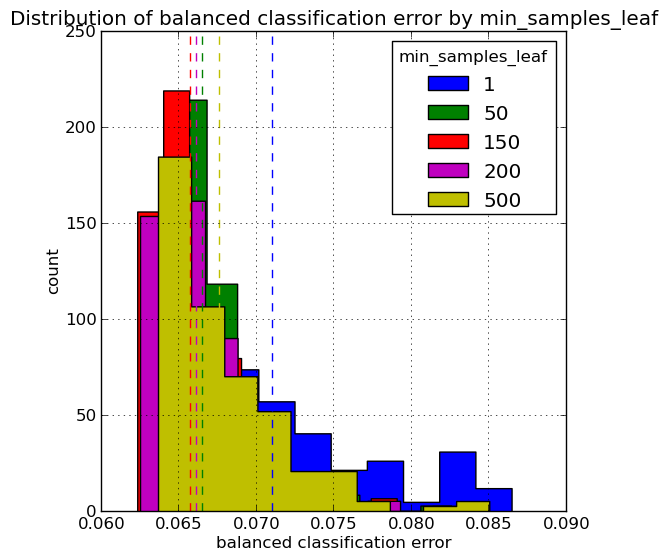
\includegraphics[scale=0.5]{Images/balanced_classification_error_min_samples_leaf.png}
%\end{figure*}
%\begin{figure*}
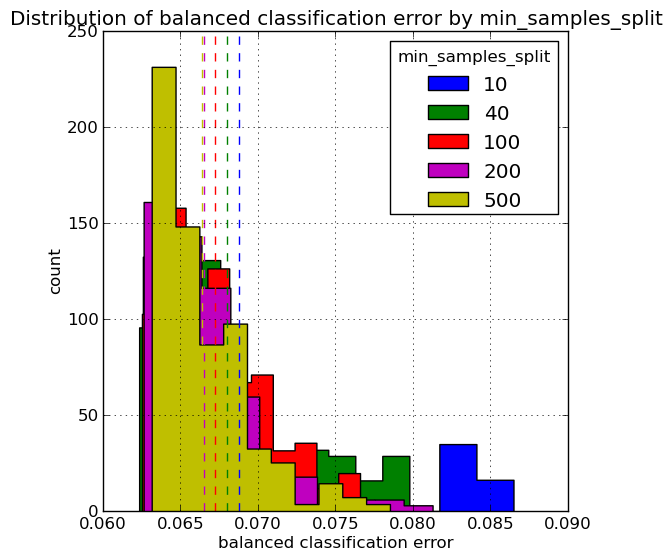
\includegraphics[scale=0.5]{Images/balanced_classification_error_min_samples_split.png}
\caption{Balanced classification error scores by parameter values}
\label{param_iterate_bce}
\end{figure*}

The table \ref{optimal_scores} summarizes the performance scores for the optimized CART tree with parameters in table \ref{param_tree}
 
\begin{table}
\centering
\begin{tabular}{l|l|l}
Metric & ROC Optimal & R(f) optimal \\
\toprule
ROC &  0.887 & 0.883\\
Precision & 0.73 & 0.72\\
Recall & 0.87 & 0.87\\
\pbox{10cm}{Balanced \\Classification Error} & 18.2\% & 18.9\%\\
AMS\footnote{The AMS is chosen at $\theta = Q_{83}, the 83rd percentile for selection region$ } & 3.31 & 2.55\\
\end{tabular}
\caption{Performance scores of the optimized DT classifier}
\label{optimal_scores}
\end{table}

\subsection{Probability Model}

We use the optimized parameters obtained in section \ref{param} to test two probability models. 

\begin{enumerate}
\item Frequency model : The conditional probability $p(y_{i}=1|\textbf{x}_{i})$ of a sample belonging to the positive signal class is the raw training frequency of the leaf node the sample ends up in, it is computed as $\dfrac{k}{n}$ where $k$ is the number of positive samples and $n$ is the total number of samples in the leaf node.  
\item Calibrated model : The probability $p(y_{i}=1|\textbf{x}_{i})$ of a sample belonging to the positive signal class is given by, $\frac{\displaystyle k + b.m}{\displaystyle n + m}$ where $b$ is the unconditional probability of the positive signal class and $m$ is a parameter that controls how much the training frequencies are skewed towards the base rate.
\end{enumerate}

The graph \ref{prob_compare} shows the probability distribution of the optimized tree applied to test set TEST. We can observe how in the frequency model of probability estimation the probabilities cluster around 0 and 1, this is due to overestimation of class probabilities as discussed in \ref{prob_calib}. 

On the other hand, the calibrated probability estimates cluster around the base rate $b$ for the positive signal class specified a priori. In many classification domains smoothing of probabilities towards the unconditional class probability could be useful. 

\begin{figure*}
\hspace{-1cm}
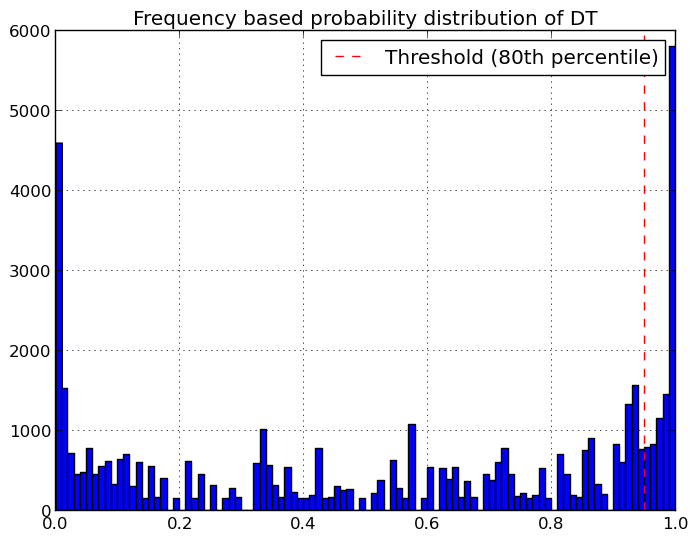
\includegraphics[scale=0.5]{Images/Prob_model.png}
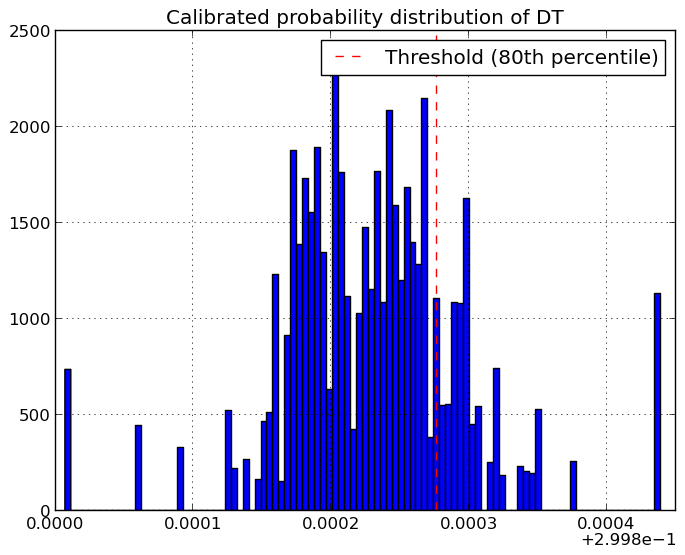
\includegraphics[scale=0.5]{Images/Prob_calib.png}
\caption{Probability calibrations under two different techniques. Base rate $b$ = 0.3 was chosen for the positive signal class.}
\label{prob_compare}
\end{figure*}

Fig. \ref{ams_compare} shows the AMS performance of the optimized CART tree computed under the two different probability models. 

\begin{figure}
%\hspace{-1cm}
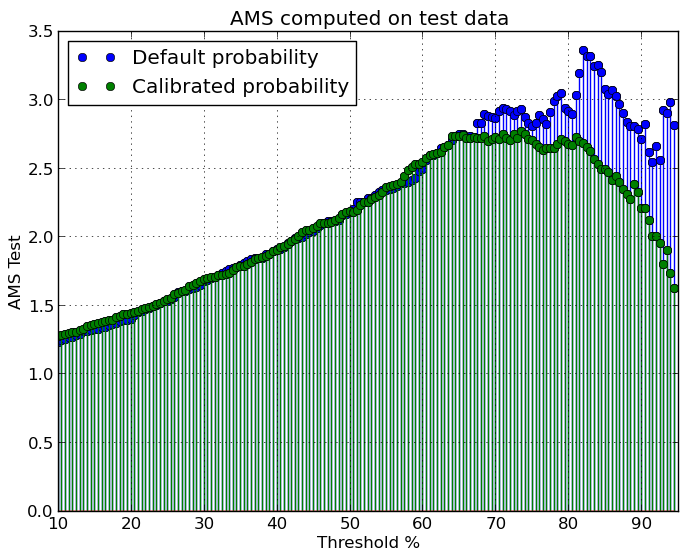
\includegraphics[scale=0.5]{Images/AMS_Probability_Compare.png}
\caption{AMS computed using the optimized parameters under the frequency model of probability (blue) and the calibrated model (green)}
\label{ams_compare}
\end{figure}

We observe that in the Higgs dataset the probability model of assigning raw training frequency as the probability scores achieves a higher AMS across the typical 70\% - 90\% thresholds. Peak AMS of 3.31 is achieved at at threshold of 84.2\%. It is interesting to note how the procedure of calibrating probability thresholds around the base rate of the signal class $b=0.3$ weakens the AMS score. 

%Since the AMS is essentially a ratio of true positives to false positives, it could be that 
%\subsection{Calibrated probabilities on the Higgs dataset}     

\section{SVM vs. Probabilistic Decision Tree}
\label{compare}

The tables \ref{compare_models} and \ref{cv_compare} compare the performance of the optimized SVM and CART classifier on the Higgs dataset. While it is apparent that the DT approach is much more scalable than the SVM, the latter is as good as the optimized CART in terms of predictive power and classification accuracy.  

\begin{table}
\begin{tabular}{l|l|l}
& SVM & CART \\
\toprule
Size of TRAIN set & 10000 & 51208\\
No. of features  & 26 & 26\\
Normalization &  Yes & No\\
Sampling applied & Yes & No \\
Optimized AMS & 3.38 & 3.31\\
ROC AUC & 0.87 & 0.908 \\
\pbox{10cm}{Balanced Classification \\Error } &0.002 & 0.06
\end{tabular}
\caption{Comparison of the SVM and CART approach on the Higgs dataset. The optimized AMS has been computed after averaging AMS scores in across a range of thresholds and accounting for their standard deviation}
\label{compare_models}
\end{table}

\begin{table}
\begin{tabular}{l|l|l}
& SVM & CART \\
\toprule
CV Runtime & 11.3 mins & 63 mins\\
Parameters to optimize & 2 & 5\\
No.of folds & 3 & 3 \\
No. of fits & 225 & 2700\\
Size of parameter grid & 75 & 900 \\ 
\end{tabular}
\caption{Cross-validation metrics}
\label{cv_compare}
\end{table}

\section{Review of Tree Algorithms}

It is worth mentioning two other tree algorithms with subtle differences to CART. ID3 (short for Iternative Dichotomizer) was a DT implementation developed by Ross Quinlan (1986) and was the precursor to the C4.5 algorithm.  For ID3, the primary difference to CART is that at each iteration it only considers the set of unused attributes to split on. It employs a greedy approach making the best choice at each split but does not guarantee a global optimum. The C4.5 iteration by Quinlan adds several enhancements to ID3. It employs a pruning procedure post tree creation which is a bottom-up technique that starts by examining leaves and prunes nodes where the reduction in impurity was below a threshold. Further, it allows differential weighting to be applied to features reflecting their importance and incorporates this information in assessing the value of a split. 

\section{Review of Algorithms applied to the Higgs dataset}
\label{lit}
There have been several successful attempts to build classifiers for the Higgs dataset used in this paper. A review of the learners used on this dataset does not indicate a clear preference for any one type of algorithm or strategy, the best published AMS score of 3.81 was attained by Gabor Melis, it uses an ensemble of deep neural networks (DNNs) with identical hyper parameters, the networks only differed in their initialization sets \cite{Gabor}. Gradient Boosting techniques were a popular choice. Many of the solutions used the \textit{XGBoost} implementation of boosted decision trees. The primary advantage of this algorithm over standard gradient boosting relied on the way the algorithm implemented regularization instead of parameter search to prune greedy CART trees.  The second place winner Tim Salimans uses a decision tree approach with regularization and constructs an ensemble of such trees, in essence a \cite{Tim} forest. It is derived from the Regularized Greedy Forest (RGF) algorithm \cite{RGF}. One of the other top teams used an ensemble approach merging the outputs of several models into one score, it used gradient boosting using XGBoost, RGF and DNN models. 

Automatic discovery of synthetic features was reportedly not very successful, on the other hand, features that were derived from the primary features based on the analytical knowledge of the underlying physics showed to improve learning performance. It is important to mention the effect of CAKE features in this respect. Derived features \textit{CakeA} and \textit{CakeB} were proposed by a team of physicists related to ATLAS. These features are generated through calculating a likelihood from first principles for the event to be a signal rather than a background. Many of the participants witnessed improved scores by incorporating this features but there was no consensus on whether the proposed feature improved scores across all learning models. 

\section{Conclusion}
The availability of the Higgs dataset in the public domain has generated great interest and curiosity about the cross-disciplinary opportunities that exist between experimental physics and machine learning. The statistical needs of the particle physics community have never been as pervasive. Physicists at CERN face a two-fold challenge, 1) a computational challenge to design classifiers that perform extremely simple yet powerful tests to reject uninteresting events as they are generated, this is so that they can minimize the size of the dataset that will have to be subjected to further deep learning and 2) a statistical challenge to design analytical measures that relate closely to generic performance metrics that classifiers are optimized on. This is necessary as classifiers that are tuned to optimize performance under accuracy metrics should concomitantly give better discovery significance. Whether or not deep learning can be used as a generalized technique to improve discovery significance in some of the most challenging questions surrounding particle physics continues to be an open one. There are hints that it could. 

\section*{Acknowledgements}

I acknowledge the assistance of my supervisor Dr. Anita Faul for advice on the content and structure of this paper and Dr. Christopher Lester who helped with understanding the physics goal of the problem. 

\section*{References}
\bibliography{References_BDT} 
\bibliographystyle{elsart-num-names.bst}

\appendix

\section{Invariant mass principle}

\label{AppA}

This section is based on \cite{RM}.

A fundamental equation of special relativity is, $$ E^2 = p^2c^2 + m^2c^4 $$ where $E$ is the energy of the particle, $p$ is its momentum, $m$ is the mass and $c$ is the speed of light. When a particle is at rest its momentum is 0, this gives us Einstein's mass-energy equivalence, $E = mc^2$.  Using the units GeV for Energy, GeV$/c$ for momentum and GeV$/c^2$ for mass we get the equivalence,  $$E^2 = p^2 + m^2 $$ The papers published in the ATLAS and CMS experiment use the notation GeV for mass, energy and momentum. We will follow the same convention.

The momentum $p$ of a particle is actually a 3-dimensional vector $\overrightarrow{p} = (p_{x}, p_{y}, p_{z})$ stating the particle's momentum in 3 directions in 3-d space. For a particle with non-zero mass the momentum of a particle is $\overrightarrow{p} = m\overrightarrow{v}$ where $\overrightarrow{v}$ is the 3-dimensional velocity and $m$ is the mass. The 4-momentum of a particle is defined as $(p_{x}, p_{y}, p_{z}, E)$. This defines the full kinematics of a particle as if we know the particle's momentum and energy we can compute its mass using the relation, $$ m = \sqrt{E^2 - p^2} $$

Similarly, if we know any two quantities out of momentum, mass and energy we can compute the third deterministically by equations of special relativity specified above. 

The mass of a particle is an intrinsic property of a particle, further by the law of conservation of energy and momentum the mass of a particle is equivalent to the mass of its decayed products each of which can be represented by their 4-momentum. For example, a particle $\chi$ decays into two final state particles $a$ and $b$ whose kinematics are captured in the detector. By conservation of energy and momentum, $$E_{\chi} = E_{a} + E_{b}$$ $$\overrightarrow{p_{\chi}} = \overrightarrow{p_{a}} + \overrightarrow{p_{b}}$$

The sum of energies and momenta of particles $a$ and $b$ should resolve to give the energy and momenta of the parent particle. The mass of the parent particle is then calculated as, $$ m_{\chi} = \sqrt{E_{\chi}^2 - p_{\chi}^2} $$ 

This is the \textit{invariant mass principle} in classical mechanics. It holds for all particles including the Higgs boson and can be generalised to more than two final states and holds in every intermediate stage of decay.   


\section{Description of Features}

\subsection{Primary Features}
\label{Pfeatures}

In the 3-d reference frame, we assume the z-axis to be the horizontal beam line. Transverse quantities are quantities projected on the plane perpendicular to the beam line, this is the $x-y$ plane. We stated earlier that the primary ingredients needed to compute the characteristics of the parent particle are the 4-momentum vectors $(p_{x}, p_{y}, p_{z}, E)$ for each of the decay products. The primary features in our dataset are quantities derived from the raw 4-momentum coordinates. These physical quantities constructed by ATLAS physicsts capture properties of the decay channel most critical to the inference of the parent particle. Below we describe these quantities which are used as features in our problem. The dataset comprises these quantities for each particle in the final-state of the collision. \cite{RM}

\textbf{Pseudorapidity ($\eta$)} : This describes the angle of the particle relative to the beam axis. It is defined as, $$ \eta = -ln [\tan(\theta/2)]$$ where $\theta$ denotes the angle between the particle and the positive direction of the beam axis. The diagram below depicts the concept, 

\begin{center}
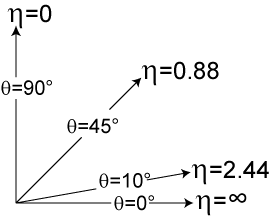
\includegraphics[scale=0.7]{Images/Pseudorapidity2.png}
\end{center}

$\eta = 0 $ corresponds to a particle in the $x-y$ plane perpendicular to the beam line, $\eta = +\infty$ corresponds to a particle travelling along the z-axis in the positive direction and $\eta = -\infty$ denotes travel in the opposite direction. Particles with high $\eta$ are usually lost and not captured by the detector. 

Particles can be identified in the range $\eta \in [-2.5 +2.5]$, for $|\eta| \in [2.5,5]$, their momentum can be measured but the particle cannot be identified. Particles with $|\eta| > 5$ escape detection all together \cite{RM}. 

\textbf{Azimuth Angle ($\phi$)} : Decay particles shoot out from the vertex of the collision which lies on the z-axis. The vector from the vertex to the particle is projected onto the transverse plane ($x-y$), the angle between the projected vector and the $x$-axis is the azimuth angle. 

\textbf{Transverse momentum  ($t$)} : The transverse momentum can be defined as the momentum that materializes in the $x-y$ plane perpendicular to the beam axis. A hard collision event is characterized by a high $t$, while proton collisions that result from protons brushing against each other leave decay particles not too far from the beam axis resulting in a small $t$. 

The transverse momentum is computed as, $$ t = \sqrt{p_{x}^2 + p_{y}^2}$$.
  
\end{document}